\documentclass{beamer}
\usepackage{tikz}
\usetheme{Warsaw}
\usepackage{graphicx}

\setbeamertemplate{footline}[frame number]
\title{Barrington's Theorem}
\author{Malek Alsalamat}
\institute{Universität Kassel}

\begin{document}

\begin{frame}
\titlepage
\end{frame}

%%%%%%%%%%%%%%%%%%%%%%%%%%%%%%%%%%%%%%%%%%%
%%%%%%%%%%%%%%%%%%%%%%%%%%%%%%%%%%%%%%%%%%%
\begin{frame}{Inhalt der Präsentation}
In der Präsentation werden wir folgends behandeln: \\[7pt]
\begin{enumerate}
\item Arten von Berechnungsmodelle \\[7pt]
\item Branching-Programme \\[7pt]
\item Zyklische Permutation \\[7pt]
\item Permutation Branching-Programme \\[7pt]
\item Beweis von Barrington Theorem
\end{enumerate}
\end{frame}


%%%%%%%%%%%%%%%%%%%%%%%%%%%%%%%%%%%%%%%%%%%
%%%%%%%%%%%%%%%%%%%%%%%%%%%%%%%%%%%%%%%%%%%
\begin{frame}{Berechnungsmodelle}
\begin{figure}[h]
\begin{center}
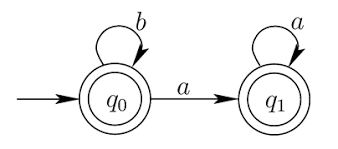
\includegraphics[width=5cm]{NFA.png}
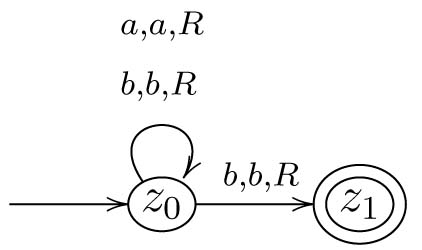
\includegraphics[width=5cm]{TM.jpg}
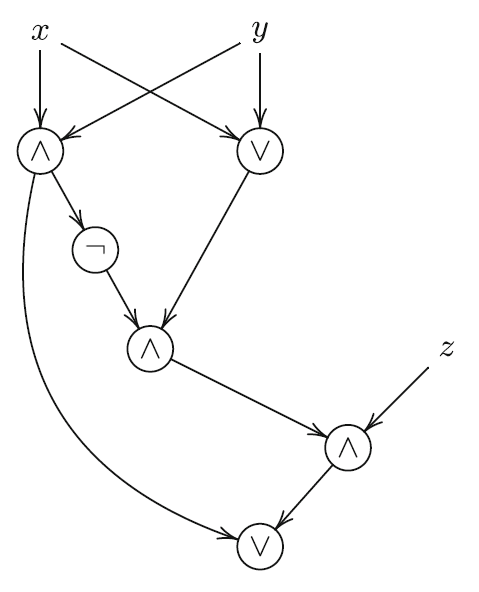
\includegraphics[width=4cm]{DeMorgan_formel.png}
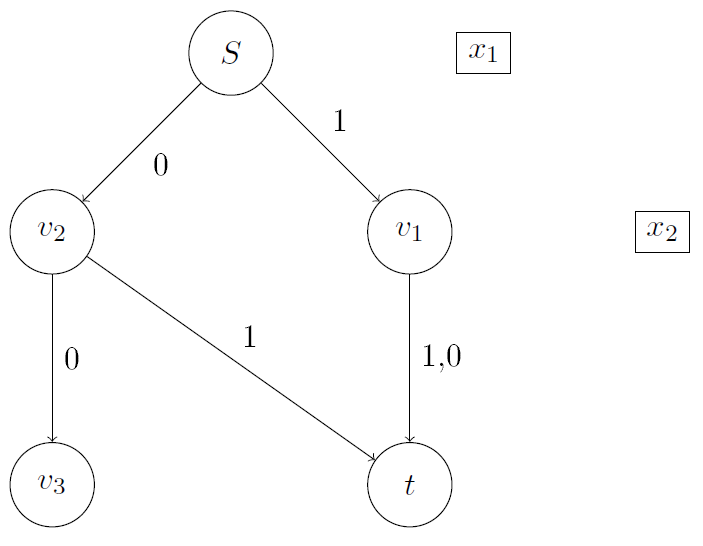
\includegraphics[width=5cm]{BP.png}
\end{center}
\end{figure}
\end{frame}



%%%%%%%%%%%%%%%%%%%%%%%%%%%%%%%%%%%%%%%%%%%%%
%%%%%%%%%%%%%%%%%%%%%%%%%%%%%%%%%%%%%%%%%%%%%
\begin{frame}{Branching-Programme}
\begin{block}{Definition von Branching-Programm}
Ein n-input Branching-Programm ist ein Tupel $P$ = ($V$,$E_0$,$E_1$,$\vartheta_0$,$t$), wobei: \\[4pt]
\begin{itemize}
\item ($V$,$E$) ist eine endliche gerichtete Graph und jeder Knote hat \textbf{fanout} 0 or 2. Wobei $E$ ist $E_0\cup E_1$.
\item $E_0$ : ist die Mengen alle Kanten, die mit 0 beschriftet sind.
\item $E_1$ : ist die Mengen alle Kanten, die mit 1 beschriftet sind.
\item $\vartheta_0$ $\in$ $V$ ist der $Startknote$.
\item $t$ ist der akzeptierende Knote ( $Endknote$ ). In folgenden wird der Startknote mit $S$ bezeichnet.  
\end{itemize}
Die berechnete Funktion von $P$ ist $f_p$: $\{0,1\}$ $^n$ $\rightarrow$ $\{0,1\}$. 
\end{block}
\end{frame}




%%%%%%%%%%%%%%%%%%%%%%%%%%%%%%%%%%%%%%%%%%%%%%%
%%%%%%%%%%%%%%%%%%%%%%%%%%%%%%%%%%%%%%%%%%%%%%%
\begin{frame}{Branching-Programme}
\only<1>{$Beipiel$ $1$: 2-input Branching-Programm}
\begin{tikzpicture}[->,node distance=3cm, auto]
\only<1>{
\node  (1)[draw, circle, minimum size=1cm]  {$S$};
\node  (2)[draw, circle, minimum size=1cm] [  below right of =   1] {$v_1$};
\node  (3)[draw, circle, minimum size=1cm] [  below left  of =   1] {$v_2$};
\node  (4)[draw, circle, minimum size=1cm] [  below  	    of =   2] {$t$};
\node  (5)[draw, circle, minimum size=1cm] [  below       of =   3] {$v_3$};
\node  (6)[draw, rectangle] [ right   of =   2] {$x_2$};
\node  (7)[draw, rectangle] [ right   of =   1] {$x_1$};
\path 	(1)edge node{1}(2)
		(1)edge node{0}(3)
		(2)edge node{1,0}(4)
		(3)edge node{0}(5)
		(3)edge node{1}(4);}

\only<2>{
\node  (1)[draw, circle, minimum size=1cm]  {$S$};
\node  (2)[draw, circle, minimum size=1cm] [  below right of =   1] {$v_1$};
\node  (3)[draw, circle, minimum size=1cm] [  below left  of =   1] {$v_2$};
\node  (4)[draw, circle, minimum size=1cm] [  below  	    of =   2] {$t$};
\node  (5)[draw, circle, minimum size=1cm] [  below       of =   3] {$v_3$};
\node  (6)[draw, rectangle, color=red] [ right   of =   2] {$x_2$};
\node  (7)[draw, rectangle, color=red] [ right   of =   1] {$x_1$};
\path 	(1)edge node{1}(2)
		(1)edge node{0}(3)
		(2)edge node{1,0}(4)
		(3)edge node{0}(5)
		(3)edge node{1}(4);}

\only<3>{
\node  (1)[draw, circle, minimum size=1cm]  {$S$};
\node  (2)[draw, circle, minimum size=1cm] [  below right of =   1] {$v_1$};
\node  (3)[draw, circle, minimum size=1cm] [  below left  of =   1] {$v_2$};
\node  (4)[draw, circle, minimum size=1cm] [  below  	    of =   2] {$t$};
\node  (5)[draw, circle, minimum size=1cm] [  below       of =   3] {$v_3$};
\node  (6)[draw, rectangle] [ right   of =   2] {$x_2$};
\node  (7)[draw, rectangle, color=red] [ right   of =   1] {$x_1=$ 1};;
\path 	(1)edge[color=red] node{1}(2)
		(1)edge node{0}(3)
		(2)edge node{1,0}(4)
		(3)edge node{0}(5)
		(3)edge node{1}(4);}				

\only<4>{
\node  (1)[draw, circle, minimum size=1cm]  {$S$};
\node  (2)[draw, circle, minimum size=1cm] [  below right of =   1] {$v_1$};
\node  (3)[draw, circle, minimum size=1cm] [  below left  of =   1] {$v_2$};
\node  (4)[draw, circle, minimum size=1cm] [  below  	    of =   2] {$t$};
\node  (5)[draw, circle, minimum size=1cm] [  below       of =   3] {$v_3$};
\node  (6)[draw, rectangle, color=red] [ right   of =   2] {$x_2=$ 0};
\node  (7)[draw, rectangle] [ right   of =   1] {$x_1$};
\path 	(1)edge node{1}(2)
		(1)edge node{0}(3)
		(2)edge[color=red] node{1,0}(4)
		(3)edge node{0}(5)
		(3)edge node{1}(4);}
		
\only<5>{
\node  (1)[draw, circle, minimum size=1cm]  {$S$};
\node  (2)[draw, circle, minimum size=1cm] [  below right of =   1] {$v_1$};
\node  (3)[draw, circle, minimum size=1cm] [  below left  of =   1] {$v_2$};
\node  (4)[draw, circle, minimum size=1cm, color=red] [  below  	    of =   2] {$t$};
\node  (5)[draw, circle, minimum size=1cm] [  below       of =   3] {$v_3$};
\node  (6)[draw, rectangle] [ right   of =   2] {$x_2$};
\node  (7)[draw, rectangle] [ right   of =   1] {$x_1$};
\path 	(1)edge node{1}(2)
		(1)edge node{0}(3)
		(2)edge node{1,0}(4)
		(3)edge node{0}(5)
		(3)edge node{1}(4);}
		
\only<6>{
\node  (1)[draw, circle, minimum size=0.7cm]  {$S$};
\node  (2)[draw, circle, minimum size=0.7cm] [  below right of =   1] {$v_1$};
\node  (3)[draw, circle, minimum size=0.7cm] [  below left  of =   1] {$v_2$};
\node  (4)[draw, circle, minimum size=0.7cm, color=red] [  below  	    of =   2] {$t$};
\node  (5)[draw, circle, minimum size=0.7cm] [  below       of =   3] {$v_3$};
\node  (6)[draw, rectangle, color=red] [ right   of =   2] {$x_2=$ 0};
\node  (7)[draw, rectangle, color=red] [ right   of =   1] {$x_1=$ 1};
\node  (8)[draw, rectangle] [right of = 4] {$input$ = $(1,0)$};
\node  (9)[draw, rectangle] [right of = 8] {$output$ = 1};
\path 	(1)edge[color=red] node{1}(2)
		(1)edge node{0}(3)
		(2)edge[color=red] node{1,0}(4)
		(3)edge node{0}(5)
		(3)edge node{1}(4);}
						
\only<7>{
\node  (1)[draw, circle, minimum size=0.7cm]  {$S$};
\node  (2)[draw, circle, minimum size=0.7cm] [  below right of =   1] {$v_1$};
\node  (3)[draw, circle, minimum size=0.7cm] [  below left  of =   1] {$v_2$};
\node  (4)[draw, circle, minimum size=0.7cm, color=red] [  below  	    of =   2] {$t$};
\node  (5)[draw, circle, minimum size=0.7cm] [  below       of =   3] {$v_3$};
\node  (6)[draw, rectangle, color=red] [ right   of =   2] {$x_2=$ 1};
\node  (7)[draw, rectangle, color=red] [ right   of =   1] {$x_1=$ 0};
\node  (8)[draw, rectangle] [right of = 4] {$input$ = $(0,1)$};
\node  (9)[draw, rectangle] [right of = 8] {$output$ = 1};
\path 	(1)edge node{1}(2)
		(1)edge[color=red] node{0}(3)
		(2)edge node{1,0}(4)
		(3)edge node{0}(5)
		(3)edge[color=red] node{1}(4);}
	
\only<8>{
\node  (1)[draw, circle, minimum size=0.7cm]  {$S$};
\node  (2)[draw, circle, minimum size=0.7cm] [  below right of =   1] {$v_1$};
\node  (3)[draw, circle, minimum size=0.7cm] [  below left  of =   1] {$v_2$};
\node  (4)[draw, circle, minimum size=0.7cm, color=red] [  below  	    of =   2] {$t$};
\node  (5)[draw, circle, minimum size=0.7cm] [  below       of =   3] {$v_3$};
\node  (6)[draw, rectangle, color=red] [ right   of =   2] {$x_2=$ 1};
\node  (7)[draw, rectangle, color=red] [ right   of =   1] {$x_1=$ 1};
\node  (8)[draw, rectangle] [right of = 4] {$input$ = $(1,1)$};
\node  (9)[draw, rectangle] [right of = 8] {$output$ = 1};
\path 	(1)edge[color=red] node{1}(2)
		(1)edge node{0}(3)
		(2)edge[color=red] node{1,0}(4)
		(3)edge node{0}(5)
		(3)edge node{1}(4);}
		
\only<9>{
\node  (1)[draw, circle, minimum size=0.7cm]  {$S$};
\node  (2)[draw, circle, minimum size=0.7cm] [  below right of =   1] {$v_1$};
\node  (3)[draw, circle, minimum size=0.7cm] [  below left  of =   1] {$v_2$};
\node  (4)[draw, circle, minimum size=0.7cm] [  below  	    of =   2] {$t$};
\node  (5)[draw, circle, minimum size=0.7cm, color=red] [  below       of =   3] {$v_3$};
\node  (6)[draw, rectangle, color=red] [ right   of =   2] {$x_2=$ 0};
\node  (7)[draw, rectangle, color=red] [ right   of =   1] {$x_1=$ 0};
\node  (8)[draw, rectangle] [right of = 4] {$input$ = $(0,0)$};
\node  (9)[draw, rectangle] [right of = 8] {$output$ = 0};
\path 	(1)edge node{1}(2)
		(1)edge[color=red] node{0}(3)
		(2)edge node{1,0}(4)
		(3)edge[color=red] node{0}(5)
		(3)edge node{1}(4);}	
\end{tikzpicture}

\only<10>{
\begin{tabular}[h]{l |c ||r}
$x_1$ & $x_2$ & $Ausgabe$\\
 \hline
0 & 0 & 0\\
0 & 1 & 1\\
1 & 0 & 1\\
1 & 1 & 1\\
\end{tabular}\\[4pt]
}

\only<11>{
\begin{tabular}[h]{l |c ||r}
$x_1$ & $x_2$ & $Ausgabe$\\
 \hline
0 & 0 & 0\\
0 & 1 & 1\\
1 & 0 & 1\\
1 & 1 & 1\\
\end{tabular}\\[4pt]
$\Rightarrow$ das Programm berechnet die $Funktion$ $f(x_1,x_2)=$ $x_1\lor x_2$.}
\end{frame}


%%%%%%%%%%%%%%%%%%%%%%%%%%%%%%%%%%%%%%%%%%%%%%%%
%%%%%%%%%%%%%%%%%%%%%%%%%%%%%%%%%%%%%%%%%%%%%%%%
\begin{frame}{Branching-Programme}
\only<1>{
Jedes Branching-Programm besitzt :
\begin{itemize}
\item Größe: Die Größe von einem Branching-Programm ist die Anzahl der Knoten in $V$ und wird mit $\mid$$V$$\mid$.
\end{itemize}
\begin{tikzpicture}[->,node distance=3cm, auto]
\node  (1)[draw, circle, minimum size=1cm, color=red]  {$S$};
\node  (2)[draw, circle, minimum size=1cm, color=red] [  below right of =   1] {$v_1$};
\node  (3)[draw, circle, minimum size=1cm, color=red] [  below left  of =   1] {$v_2$};
\node  (4)[draw, circle, minimum size=1cm, color=red] [  below  	    of =   2] {$t$};
\node  (5)[draw, circle, minimum size=1cm, color=red] [  below       of =   3] {$v_3$};
\node  (6)[draw, rectangle] [ right   of =   2] {$x_2$};
\node  (7)[draw, rectangle] [ right   of =   1] {$x_1$};
\node  (7)[draw, rectangle] [ right   of =   4] {$\Rightarrow$ $\mid V\mid$ = 5};
\path 	(1)edge node{1}(2)
		(1)edge node{0}(3)
		(2)edge node{1,0}(4)
		(3)edge node{0}(5)
		(3)edge node{1}(4);
\end{tikzpicture}
}

\only<2>{
Jedes Branching-Programm besitzt :
\begin{itemize}
\item Tiefe: Die Tiefe oder Länge von einem Branching-Programm ist der längste Pfad in unserem Graph $(V,E)$.
\end{itemize}
\begin{tikzpicture}[->,node distance=3cm, auto]
\node  (1)[draw, circle, minimum size=1cm]  {$S$};
\node  (2)[draw, circle, minimum size=1cm] [  below right of =   1] {$v_1$};
\node  (3)[draw, circle, minimum size=1cm] [  below left  of =   1] {$v_2$};
\node  (4)[draw, circle, minimum size=1cm] [  below  	    of =   2] {$t$};
\node  (5)[draw, circle, minimum size=1cm] [  below       of =   3] {$v_3$};
\node  (6)[draw, rectangle] [ right   of =   2] {$x_2$};
\node  (7)[draw, rectangle] [ right   of =   1] {$x_1$};
\path 	(1)edge[color=red] node{1}(2)
		(1)edge node{0}(3)
		(2)edge[color=red] node{1,0}(4)
		(3)edge node{0}(5)
		(3)edge node{1}(4);
\end{tikzpicture}
}

\only<3>{
Jedes Branching-Programm besitzt :
\begin{itemize}
\item Tiefe: Die Tiefe oder Länge von einem Branching-Programm ist der längste Pfad in unserem Graph $(V,E)$.
\end{itemize}
\begin{tikzpicture}[->,node distance=3cm, auto]
\node  (1)[draw, circle, minimum size=1cm]  {$S$};
\node  (2)[draw, circle, minimum size=1cm] [  below right of =   1] {$v_1$};
\node  (3)[draw, circle, minimum size=1cm] [  below left  of =   1] {$v_2$};
\node  (4)[draw, circle, minimum size=1cm] [  below  	    of =   2] {$t$};
\node  (5)[draw, circle, minimum size=1cm] [  below       of =   3] {$v_3$};
\node  (6)[draw, rectangle] [ right   of =   2] {$x_2$};
\node  (7)[draw, rectangle] [ right   of =   1] {$x_1$};
\path 	(1)edge node{1}(2)
		(1)edge[color=red] node{0}(3)
		(2)edge node{1,0}(4)
		(3)edge[color=red] node{0}(5)
		(3)edge node{1}(4);
\end{tikzpicture}
}

\only<4>{
Jedes Branching-Programm besitzt :
\begin{itemize}
\item Tiefe: Die Tiefe oder Länge von einem Branching-Programm ist der längste Pfad in unserem Graph $(V,E)$.
\end{itemize}
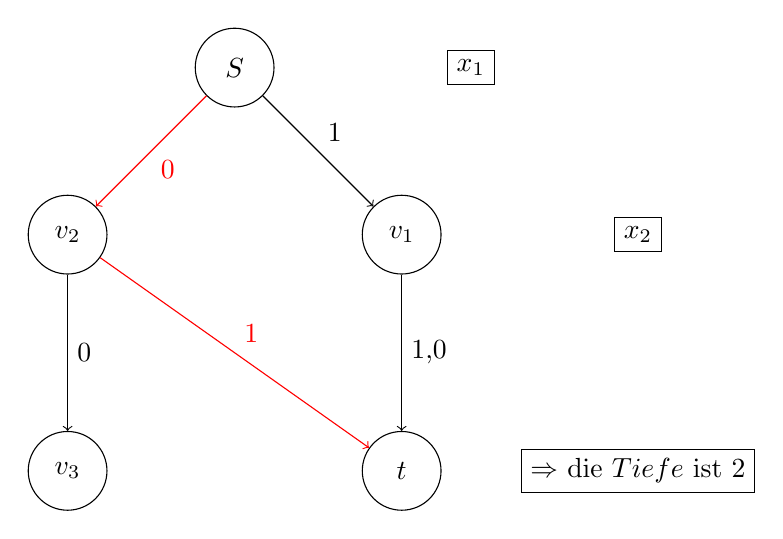
\begin{tikzpicture}[->,node distance=3cm, auto]
\node  (1)[draw, circle, minimum size=1cm]  {$S$};
\node  (2)[draw, circle, minimum size=1cm] [  below right of =   1] {$v_1$};
\node  (3)[draw, circle, minimum size=1cm] [  below left  of =   1] {$v_2$};
\node  (4)[draw, circle, minimum size=1cm] [  below  	    of =   2] {$t$};
\node  (5)[draw, circle, minimum size=1cm] [  below       of =   3] {$v_3$};
\node  (6)[draw, rectangle] [ right   of =   2] {$x_2$};
\node  (7)[draw, rectangle] [ right   of =   1] {$x_1$};
\node  (7)[draw, rectangle] [ right   of =   4] {$\Rightarrow$ die $Tiefe$ ist 2};
\path 	(1)edge node{1}(2)
		(1)edge[color=red] node{0}(3)
		(2)edge node{1,0}(4)
		(3)edge node{0}(5)
		(3)edge[color=red] node{1}(4);
\end{tikzpicture}
}

\only<5>{
Jedes Branching-Programm besitzt :
\begin{itemize}
\item Breite: Die Breite von einem Branching-Programm ist die maximale Anzahl von Knoten in einem Level.
\end{itemize}
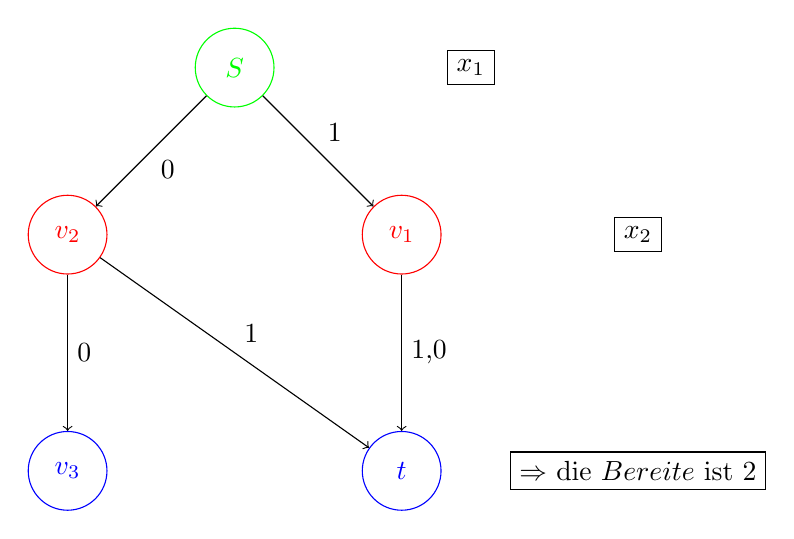
\begin{tikzpicture}[->,node distance=3cm, auto]
\node  (1)[draw, circle, minimum size=1cm, , color=green]  {$S$};
\node  (2)[draw, circle, minimum size=1cm, color=red] [  below right of =   1] {$v_1$};
\node  (3)[draw, circle, minimum size=1cm, color=red] [  below left  of =   1] {$v_2$};
\node  (4)[draw, circle, minimum size=1cm, color=blue] [  below  	    of =   2] {$t$};
\node  (5)[draw, circle, minimum size=1cm, color=blue] [  below       of =   3] {$v_3$};
\node  (6)[draw, rectangle] [ right   of =   2] {$x_2$};
\node  (7)[draw, rectangle] [ right   of =   1] {$x_1$};
\node  (7)[draw, rectangle] [ right   of =   4] {$\Rightarrow$ die $Bereite$ ist 2};
\path 	(1)edge node{1}(2)
		(1)edge node{0}(3)
		(2)edge node{1,0}(4)
		(3)edge node{0}(5)
		(3)edge node{1}(4);
\end{tikzpicture}
}
\end{frame}

%%%%%%%%%%%%%%%%%%%%%%%%%%%%%%%%%%%%%%%%%%
%%%%%%%%%%%%%%%%%%%%%%%%%%%%%%%%%%%%%%%%%%
\begin{frame}{Branching-Programme}
$Majority(x)=
\begin{cases} 
1,& \sum\nolimits_{i=0}^N x_i \ge n/2\\
0,& sonst
\end{cases}$\\[4pt]
NC = $\bigcup_{i=0}^\infty NC^{i}$. Für alle $i \in \mathbb{N}$ ist $NC^{i}$ die Klasse aller Sprachen, die von einer Schaltkreisfamilie mit polynomieller Größe, Tiefe $\mathcal{O}(log^{i}(n))$ und einen Fan-In von höchstens 2 erkannt werden.\\[4pt]
In $NC^{1}$ liegen beispielsweise die Addition und Multiplikation, sowie die Majority-Funktion.\\[4pt]
Im Jahr 1986 hat Barrington gezeigt, dass $NC^{1}$ = 5-BP. Und dadurch gezeigt, dass die Majority-Funktion durch solche BP berechnet werden können.
\end{frame}

%%%%%%%%%%%%%%%%%%%%%%%%%%%%%%%%%%%%%%%%%%
%%%%%%%%%%%%%%%%%%%%%%%%%%%%%%%%%%%%%%%%%%

\begin{frame}{Zyklische Permutation}
\begin{block}{Permutationen}
Eine Permutation von $\{1,\dots,n\}$ ist eine bijektive Abbildung\\ $\sigma$ : $\{1,\dots,n\}$ $\rightarrow$ $\{1,\dots,n\}$ , $i$ $\rightarrow$ $\sigma(i)$. \\[4pt]
%Darstellung:$\sigma$ = \left(\begin{array}{cccc} $i_1$ & $i_2$ & $\dots$ & $i_n$ \\ 
%											$\sigma(i_1)$ & $\sigma(i_1)$ & $\dots$ & $\sigma(i_n)$
%\end{array}\right)
Zyklische Schreibweiße = ($i_1$,$\sigma(i_1)$, $\sigma(\sigma(i_{1}))$,\dots).\\[4pt]
Eine Permutation heißt zyklisch wenn : \[ \sigma(i_j) = \left\{\begin{array}{cl}i_1 & \mbox{  $j=n$} \\i_{j+1} & \mbox{  sonst}\end{array} \right. \]
Beispiele:
\[
  a_1 = 
  \begin{pmatrix}
    1 & 2 & 3 \\
    2 & 3 & 1 
  \end{pmatrix}
\] \[
  a_2 = 
  \begin{pmatrix}
    1 & 2 & 3 & 4 & 5\\
    3 & 1 & 2 & 5 & 4
  \end{pmatrix}
\] $a_1$ = $(1,2,3)$, $a_2$ = $(1,3,2)(4,5)$ $\Rightarrow$ $a_1$ ist zyklisch, aber $a_2$ nicht.

\end{block}
\end{frame}



%%%%%%%%%%%%%%%%%%%%%%%%%%%%%%%%%%%%%%%%%%%%%%%%%%%%%%
%%%%%%%%%%%%%%%%%%%%%%%%%%%%%%%%%%%%%%%%%%%%%%%%%%%%%%
\begin{frame}{Permutation Branching-Programm}

Ein w-Permutation Branching-Programm ist ein BP mit folgende Eigenschaften:
\begin{itemize}
\item Jedes Level hat genau w Knoten und somit ist die Bereite w.
\item Jedes Level ist mit der selben Variable beschriftet.
\item Die Verbindung zwischen zwei Levels realisieren Permutationen von Typ [w] $\rightarrow$ [w]. Wobei [w] ist $\{1,\dots,w\}$.
\item Jeder Knote $v$ aus dem $Level_i$ wird mit dem Input 0 oder 1 nur auf Knoten aus dem $Level_{i+1}$ abgebildet. Kurz gesagt, das Programm liegt in Schichtenform.
\item Die 1-Kanten sind mit
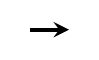
\begin{tikzpicture} 
\draw[arrows=-stealth, line width=0.5mm] (0,0) -- (0.5,0);
\end{tikzpicture}
bezeichnet und die 0-Kanten mit 
\begin{tikzpicture} 
\draw[->] (0,0) -- (0.5,0);
\end{tikzpicture}.  
\end{itemize}
Für eine boolesche Funktion $f$ und eine Permutation $\sigma$, sagen wir $P$ $\sigma$-berechnet $f$, falls für jedes Input x gilt: 
\[ P(x) = \left\{\begin{array}{cl} \sigma & \mbox{  , $f(x)$ = 1} \\ $e$ & \mbox{  , $f(x)$ = 0}\end{array} \right. \]
wobei e ist die identität Permutation.
\end{frame}



%%%%%%%%%%%%%%%%%%%%%%%%%%%%%%%%%%%%%%%%%%%%%%%%%%%%%%
%%%%%%%%%%%%%%%%%%%%%%%%%%%%%%%%%%%%%%%%%%%%%%%%%%%%%%
\begin{frame}{Permutation Branching Programm}
\only<1>{
$Beispiel$ 2:\\[4pt]
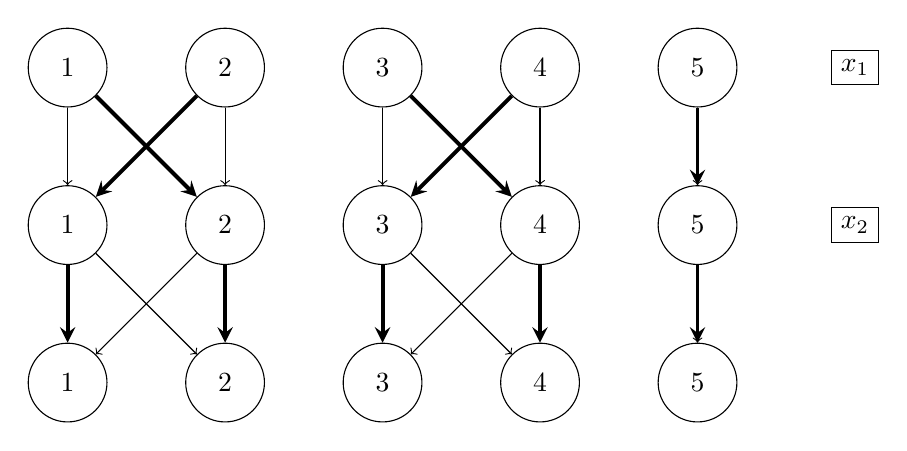
\begin{tikzpicture}[node distance=2cm, auto]
\node  (1)[draw, circle, minimum size=1cm]  {1};
\node  (2)[draw, circle, minimum size=1cm] [  right   of = 1] {2};
\node  (3)[draw, circle, minimum size=1cm] [  right  of = 2] {3};
\node  (4)[draw, circle, minimum size=1cm] [  right  of = 3] {4};
\node  (5)[draw, circle, minimum size=1cm] [  right  of = 4] {5};
\node  (x)[draw, rectangle] [  right  of = 5] {$x_1$};
\node  (6)[draw, circle, minimum size=1cm] [  below   of = 1] {1};
\node  (7)[draw, circle, minimum size=1cm] [  below  of = 2] {2};
\node  (8)[draw, circle, minimum size=1cm] [  below  of = 3] {3};
\node  (9)[draw, circle, minimum size=1cm] [  below  of = 4] {4};
\node  (10)[draw, circle, minimum size=1cm] [  below  of = 5] {5};
\node  (x)[draw, rectangle] [  right  of = 10] {$x_2$};
\node  (11)[draw, circle, minimum size=1cm] [  below   of = 6] {1};
\node  (12)[draw, circle, minimum size=1cm] [  below  of = 7] {2};
\node  (13)[draw, circle, minimum size=1cm] [  below  of = 8] {3};
\node  (14)[draw, circle, minimum size=1cm] [  below  of = 9] {4};
\node  (15)[draw, circle, minimum size=1cm] [  below  of = 10] {5};
\draw[arrows=-stealth, line width=0.5mm] (1) -- (7);
\draw[arrows=-stealth, line width=0.5mm] (2) -- (6);
\draw[arrows=-stealth, line width=0.5mm] (3) -- (9);
\draw[arrows=-stealth, line width=0.5mm] (4) -- (8);
\draw[arrows=-stealth, line width=0.5mm] (5) -- (10);
\draw[arrows=-stealth, line width=0.5mm] (7) -- (12);
\draw[arrows=-stealth, line width=0.5mm] (6) -- (11);
\draw[arrows=-stealth, line width=0.5mm] (8) -- (13);
\draw[arrows=-stealth, line width=0.5mm] (9) -- (14);
\draw[arrows=-stealth, line width=0.5mm] (10) -- (15);
\draw[->] (1) -- (6);
\draw[->] (2) -- (7);
\draw[->] (3) -- (8);
\draw[->] (4) -- (9);
\draw[->] (5) -- (10);
\draw[->] (6) -- (12);
\draw[->] (7) -- (11);
\draw[->] (8) -- (14);
\draw[->] (9) -- (13);
\draw[->] (10) -- (15);
\end{tikzpicture}}

\only<2>{
$Beispiel$ 2:\\[4pt]
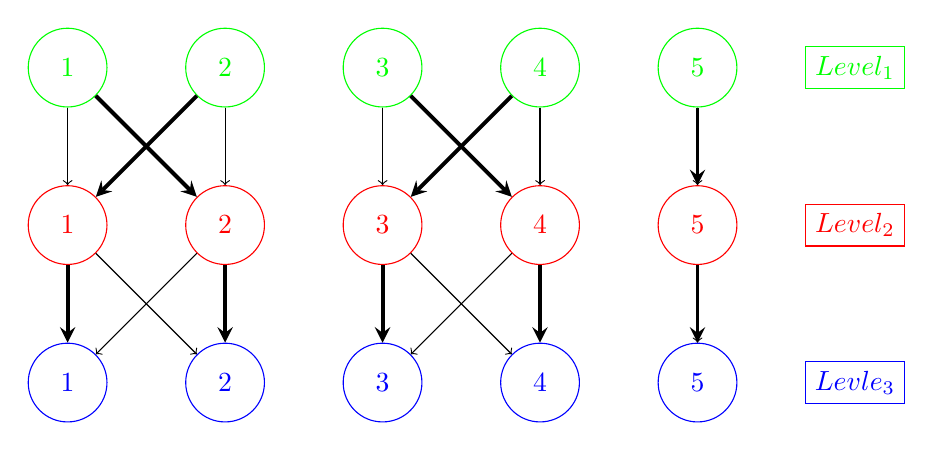
\begin{tikzpicture}[node distance=2cm, auto]
\node  (1)[draw, circle, minimum size=1cm, color=green]  {1};
\node  (2)[draw, circle, minimum size=1cm, color=green] [  right   of = 1] {2};
\node  (3)[draw, circle, minimum size=1cm, color=green] [  right  of = 2] {3};
\node  (4)[draw, circle, minimum size=1cm, color=green] [  right  of = 3] {4};
\node  (5)[draw, circle, minimum size=1cm, color=green] [  right  of = 4] {5};
\node  (x)[draw, rectangle, color=green] [  right  of = 5] {$Level_1$};
\node  (6)[draw, circle, minimum size=1cm, color=red] [  below   of = 1] {1};
\node  (7)[draw, circle, minimum size=1cm, color=red] [  below  of = 2] {2};
\node  (8)[draw, circle, minimum size=1cm, color=red] [  below  of = 3] {3};
\node  (9)[draw, circle, minimum size=1cm, color=red] [  below  of = 4] {4};
\node  (10)[draw, circle, minimum size=1cm, color=red] [  below  of = 5] {5};
\node  (x)[draw, rectangle, color=red] [  right  of = 10] {$Level_2$};
\node  (11)[draw, circle, minimum size=1cm, color=blue] [  below   of = 6] {1};
\node  (12)[draw, circle, minimum size=1cm, color=blue] [  below  of = 7] {2};
\node  (13)[draw, circle, minimum size=1cm, color=blue] [  below  of = 8] {3};
\node  (14)[draw, circle, minimum size=1cm, color=blue] [  below  of = 9] {4};
\node  (15)[draw, circle, minimum size=1cm, color=blue] [  below  of = 10] {5};
\node  (x)[draw, rectangle, color=blue] [  right  of = 15] {$Levle_3$};
\draw[arrows=-stealth, line width=0.5mm] (1) -- (7);
\draw[arrows=-stealth, line width=0.5mm] (2) -- (6);
\draw[arrows=-stealth, line width=0.5mm] (3) -- (9);
\draw[arrows=-stealth, line width=0.5mm] (4) -- (8);
\draw[arrows=-stealth, line width=0.5mm] (5) -- (10);
\draw[arrows=-stealth, line width=0.5mm] (7) -- (12);
\draw[arrows=-stealth, line width=0.5mm] (6) -- (11);
\draw[arrows=-stealth, line width=0.5mm] (8) -- (13);
\draw[arrows=-stealth, line width=0.5mm] (9) -- (14);
\draw[arrows=-stealth, line width=0.5mm] (10) -- (15);
\draw[->] (1) -- (6);
\draw[->] (2) -- (7);
\draw[->] (3) -- (8);
\draw[->] (4) -- (9);
\draw[->] (5) -- (10);
\draw[->] (6) -- (12);
\draw[->] (7) -- (11);
\draw[->] (8) -- (14);
\draw[->] (9) -- (13);
\draw[->] (10) -- (15);
\end{tikzpicture}}

\only<3>{
$Beispiel$ 2:\\[4pt]
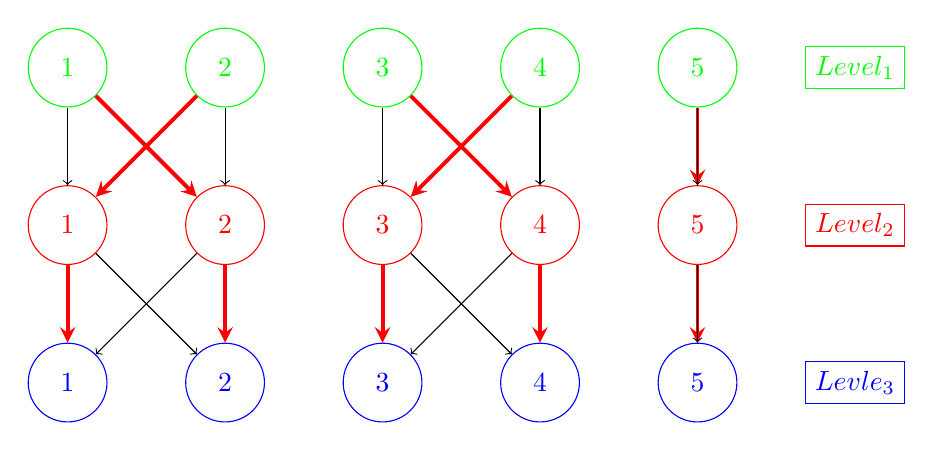
\begin{tikzpicture}[node distance=2cm, auto]
\node  (1)[draw, circle, minimum size=1cm, color=green]  {1};
\node  (2)[draw, circle, minimum size=1cm, color=green] [  right   of = 1] {2};
\node  (3)[draw, circle, minimum size=1cm, color=green] [  right  of = 2] {3};
\node  (4)[draw, circle, minimum size=1cm, color=green] [  right  of = 3] {4};
\node  (5)[draw, circle, minimum size=1cm, color=green] [  right  of = 4] {5};
\node  (x)[draw, rectangle, color=green] [  right  of = 5] {$Level_1$};
\node  (6)[draw, circle, minimum size=1cm, color=red] [  below   of = 1] {1};
\node  (7)[draw, circle, minimum size=1cm, color=red] [  below  of = 2] {2};
\node  (8)[draw, circle, minimum size=1cm, color=red] [  below  of = 3] {3};
\node  (9)[draw, circle, minimum size=1cm, color=red] [  below  of = 4] {4};
\node  (10)[draw, circle, minimum size=1cm, color=red] [  below  of = 5] {5};
\node  (x)[draw, rectangle, color=red] [  right  of = 10] {$Level_2$};
\node  (11)[draw, circle, minimum size=1cm, color=blue] [  below   of = 6] {1};
\node  (12)[draw, circle, minimum size=1cm, color=blue] [  below  of = 7] {2};
\node  (13)[draw, circle, minimum size=1cm, color=blue] [  below  of = 8] {3};
\node  (14)[draw, circle, minimum size=1cm, color=blue] [  below  of = 9] {4};
\node  (15)[draw, circle, minimum size=1cm, color=blue] [  below  of = 10] {5};
\node  (x)[draw, rectangle, color=blue] [  right  of = 15] {$Levle_3$};
\draw[arrows=-stealth, line width=0.5mm, color=red] (1) -- (7);
\draw[arrows=-stealth, line width=0.5mm, color=red] (2) -- (6);
\draw[arrows=-stealth, line width=0.5mm, color=red] (3) -- (9);
\draw[arrows=-stealth, line width=0.5mm, color=red] (4) -- (8);
\draw[arrows=-stealth, line width=0.5mm, color=red] (5) -- (10);
\draw[arrows=-stealth, line width=0.5mm, color=red] (7) -- (12);
\draw[arrows=-stealth, line width=0.5mm, color=red] (6) -- (11);
\draw[arrows=-stealth, line width=0.5mm, color=red] (8) -- (13);
\draw[arrows=-stealth, line width=0.5mm, color=red] (9) -- (14);
\draw[arrows=-stealth, line width=0.5mm, color=red] (10) -- (15);
\draw[->] (1) -- (6);
\draw[->] (2) -- (7);
\draw[->] (3) -- (8);
\draw[->] (4) -- (9);
\draw[->] (5) -- (10);
\draw[->] (6) -- (12);
\draw[->] (7) -- (11);
\draw[->] (8) -- (14);
\draw[->] (9) -- (13);
\draw[->] (10) -- (15);
\end{tikzpicture}}


\only<4>{
$Beispiel$ 2:\\[4pt]
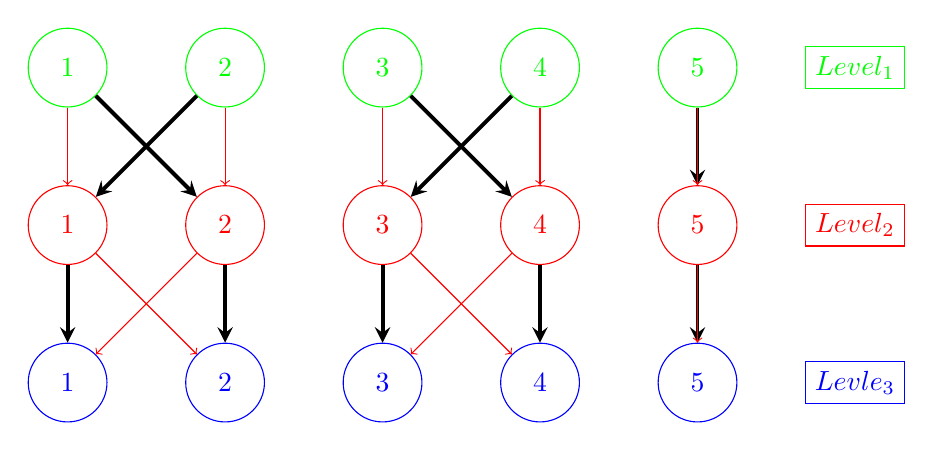
\begin{tikzpicture}[node distance=2cm, auto]
\node  (1)[draw, circle, minimum size=1cm, color=green]  {1};
\node  (2)[draw, circle, minimum size=1cm, color=green] [  right   of = 1] {2};
\node  (3)[draw, circle, minimum size=1cm, color=green] [  right  of = 2] {3};
\node  (4)[draw, circle, minimum size=1cm, color=green] [  right  of = 3] {4};
\node  (5)[draw, circle, minimum size=1cm, color=green] [  right  of = 4] {5};
\node  (x)[draw, rectangle, color=green] [  right  of = 5] {$Level_1$};
\node  (6)[draw, circle, minimum size=1cm, color=red] [  below   of = 1] {1};
\node  (7)[draw, circle, minimum size=1cm, color=red] [  below  of = 2] {2};
\node  (8)[draw, circle, minimum size=1cm, color=red] [  below  of = 3] {3};
\node  (9)[draw, circle, minimum size=1cm, color=red] [  below  of = 4] {4};
\node  (10)[draw, circle, minimum size=1cm, color=red] [  below  of = 5] {5};
\node  (x)[draw, rectangle, color=red] [  right  of = 10] {$Level_2$};
\node  (11)[draw, circle, minimum size=1cm, color=blue] [  below   of = 6] {1};
\node  (12)[draw, circle, minimum size=1cm, color=blue] [  below  of = 7] {2};
\node  (13)[draw, circle, minimum size=1cm, color=blue] [  below  of = 8] {3};
\node  (14)[draw, circle, minimum size=1cm, color=blue] [  below  of = 9] {4};
\node  (15)[draw, circle, minimum size=1cm, color=blue] [  below  of = 10] {5};
\node  (x)[draw, rectangle, color=blue] [  right  of = 15] {$Levle_3$};
\draw[arrows=-stealth, line width=0.5mm] (1) -- (7);
\draw[arrows=-stealth, line width=0.5mm] (2) -- (6);
\draw[arrows=-stealth, line width=0.5mm] (3) -- (9);
\draw[arrows=-stealth, line width=0.5mm] (4) -- (8);
\draw[arrows=-stealth, line width=0.5mm] (5) -- (10);
\draw[arrows=-stealth, line width=0.5mm] (7) -- (12);
\draw[arrows=-stealth, line width=0.5mm] (6) -- (11);
\draw[arrows=-stealth, line width=0.5mm] (8) -- (13);
\draw[arrows=-stealth, line width=0.5mm] (9) -- (14);
\draw[arrows=-stealth, line width=0.5mm] (10) -- (15);
\draw[-> , color=red] (1) -- (6);
\draw[->, color=red] (2) -- (7);
\draw[->, color=red] (3) -- (8);
\draw[->, color=red] (4) -- (9);
\draw[->, color=red] (5) -- (10);
\draw[->, color=red] (6) -- (12);
\draw[->, color=red] (7) -- (11);
\draw[->, color=red] (8) -- (14);
\draw[->, color=red] (9) -- (13);
\draw[->, color=red] (10) -- (15);
\end{tikzpicture}}


\only<5>{
Was berechnet $P$? und was passiert auf die Eingabe (0,0)? \\[4pt]
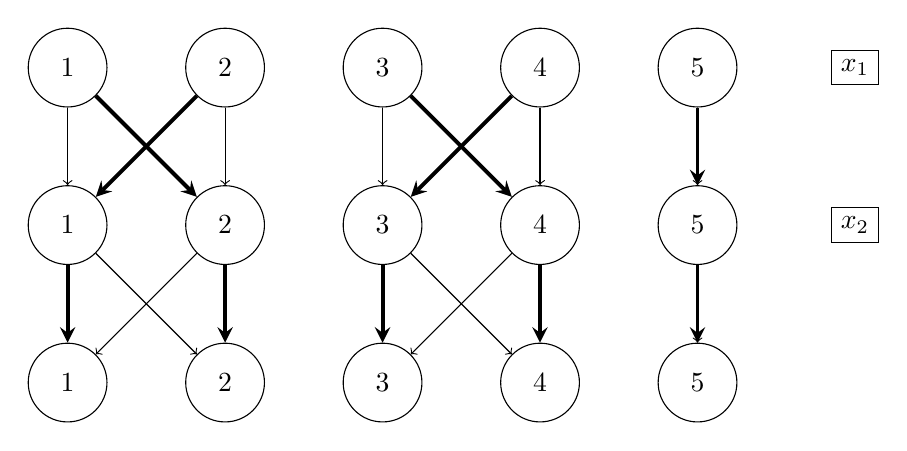
\begin{tikzpicture}[node distance=2cm, auto]
\node  (1)[draw, circle, minimum size=1cm]  {1};
\node  (2)[draw, circle, minimum size=1cm] [  right   of = 1] {2};
\node  (3)[draw, circle, minimum size=1cm] [  right  of = 2] {3};
\node  (4)[draw, circle, minimum size=1cm] [  right  of = 3] {4};
\node  (5)[draw, circle, minimum size=1cm] [  right  of = 4] {5};
\node  (x)[draw, rectangle] [  right  of = 5] {$x_1$};
\node  (6)[draw, circle, minimum size=1cm] [  below   of = 1] {1};
\node  (7)[draw, circle, minimum size=1cm] [  below  of = 2] {2};
\node  (8)[draw, circle, minimum size=1cm] [  below  of = 3] {3};
\node  (9)[draw, circle, minimum size=1cm] [  below  of = 4] {4};
\node  (10)[draw, circle, minimum size=1cm] [  below  of = 5] {5};
\node  (x)[draw, rectangle] [  right  of = 10] {$x_2$};
\node  (11)[draw, circle, minimum size=1cm] [  below   of = 6] {1};
\node  (12)[draw, circle, minimum size=1cm] [  below  of = 7] {2};
\node  (13)[draw, circle, minimum size=1cm] [  below  of = 8] {3};
\node  (14)[draw, circle, minimum size=1cm] [  below  of = 9] {4};
\node  (15)[draw, circle, minimum size=1cm] [  below  of = 10] {5};
\draw[arrows=-stealth, line width=0.5mm] (1) -- (7);
\draw[arrows=-stealth, line width=0.5mm] (2) -- (6);
\draw[arrows=-stealth, line width=0.5mm] (3) -- (9);
\draw[arrows=-stealth, line width=0.5mm] (4) -- (8);
\draw[arrows=-stealth, line width=0.5mm] (5) -- (10);
\draw[arrows=-stealth, line width=0.5mm] (7) -- (12);
\draw[arrows=-stealth, line width=0.5mm] (6) -- (11);
\draw[arrows=-stealth, line width=0.5mm] (8) -- (13);
\draw[arrows=-stealth, line width=0.5mm] (9) -- (14);
\draw[arrows=-stealth, line width=0.5mm] (10) -- (15);
\draw[->] (1) -- (6);
\draw[->] (2) -- (7);
\draw[->] (3) -- (8);
\draw[->] (4) -- (9);
\draw[->] (5) -- (10);
\draw[->] (6) -- (12);
\draw[->] (7) -- (11);
\draw[->] (8) -- (14);
\draw[->] (9) -- (13);
\draw[->] (10) -- (15);
\end{tikzpicture}}


\only<6>{
Die Permutation für zwischen ersten und zweiten Level: \\[4pt]
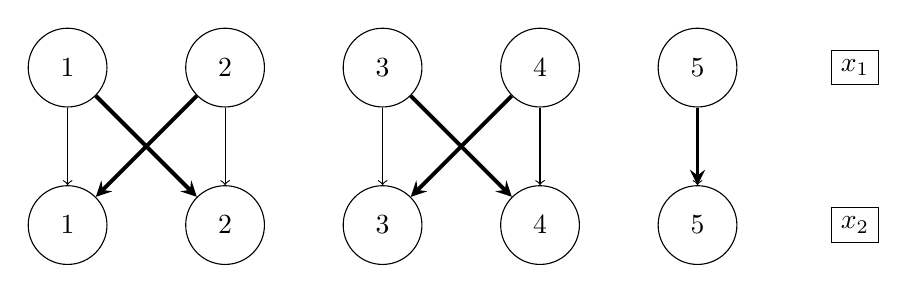
\begin{tikzpicture}[node distance=2cm, auto]
\node  (1)[draw, circle, minimum size=1cm]  {1};
\node  (2)[draw, circle, minimum size=1cm] [  right   of = 1] {2};
\node  (3)[draw, circle, minimum size=1cm] [  right  of = 2] {3};
\node  (4)[draw, circle, minimum size=1cm] [  right  of = 3] {4};
\node  (5)[draw, circle, minimum size=1cm] [  right  of = 4] {5};
\node  (x)[draw, rectangle] [  right  of = 5] {$x_1$};
\node  (6)[draw, circle, minimum size=1cm] [  below   of = 1] {1};
\node  (7)[draw, circle, minimum size=1cm] [  below  of = 2] {2};
\node  (8)[draw, circle, minimum size=1cm] [  below  of = 3] {3};
\node  (9)[draw, circle, minimum size=1cm] [  below  of = 4] {4};
\node  (10)[draw, circle, minimum size=1cm] [  below  of = 5] {5};
\node  (x)[draw, rectangle] [  right  of = 10] {$x_2$};
\draw[arrows=-stealth, line width=0.5mm] (1) -- (7);
\draw[arrows=-stealth, line width=0.5mm] (2) -- (6);
\draw[arrows=-stealth, line width=0.5mm] (3) -- (9);
\draw[arrows=-stealth, line width=0.5mm] (4) -- (8);
\draw[arrows=-stealth, line width=0.5mm] (5) -- (10);
\draw[->] (1) -- (6);
\draw[->] (2) -- (7);
\draw[->] (3) -- (8);
\draw[->] (4) -- (9);
\draw[->] (5) -- (10);
\end{tikzpicture}}


\only<7>{
Die Permutation für $1-Kanten$ zwischen dem ersten und zweiten Level:\\[4pt]
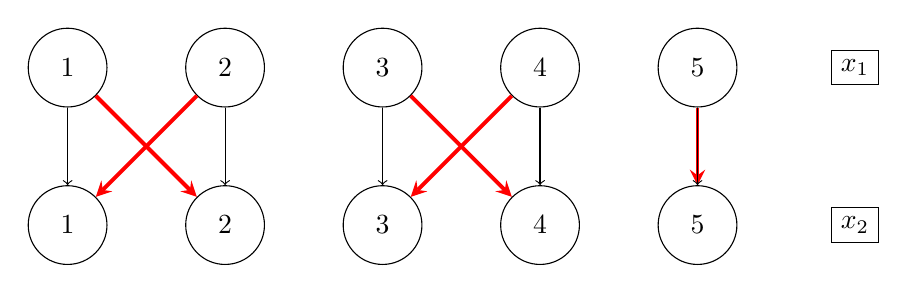
\begin{tikzpicture}[node distance=2cm, auto]
\node  (1)[draw, circle, minimum size=1cm]  {1};
\node  (2)[draw, circle, minimum size=1cm] [  right   of = 1] {2};
\node  (3)[draw, circle, minimum size=1cm] [  right  of = 2] {3};
\node  (4)[draw, circle, minimum size=1cm] [  right  of = 3] {4};
\node  (5)[draw, circle, minimum size=1cm] [  right  of = 4] {5};
\node  (x)[draw, rectangle] [  right  of = 5] {$x_1$};
\node  (6)[draw, circle, minimum size=1cm] [  below   of = 1] {1};
\node  (7)[draw, circle, minimum size=1cm] [  below  of = 2] {2};
\node  (8)[draw, circle, minimum size=1cm] [  below  of = 3] {3};
\node  (9)[draw, circle, minimum size=1cm] [  below  of = 4] {4};
\node  (10)[draw, circle, minimum size=1cm] [  below  of = 5] {5};
\node  (x)[draw, rectangle] [  right  of = 10] {$x_2$};
\draw[arrows=-stealth, line width=0.5mm, color=red] (1) -- (7);
\draw[arrows=-stealth, line width=0.5mm, color=red] (2) -- (6);
\draw[arrows=-stealth, line width=0.5mm, color=red] (3) -- (9);
\draw[arrows=-stealth, line width=0.5mm, color=red] (4) -- (8);
\draw[arrows=-stealth, line width=0.5mm, color=red] (5) -- (10);
\draw[->] (1) -- (6);
\draw[->] (2) -- (7);
\draw[->] (3) -- (8);
\draw[->] (4) -- (9);
\draw[->] (5) -- (10);
\end{tikzpicture}
\[
  \sigma_1  = 
  \begin{pmatrix}
    1 & 2 & 3 & 4 & 5 \\
    2 & 1 & 4 & 3 & 5 
  \end{pmatrix} = (1,2)(3,4)(5)
\]}


\only<8>{
Die Permutation für $0-Kanten$ zwischen dem ersten und zweiten Level:\\[4pt]
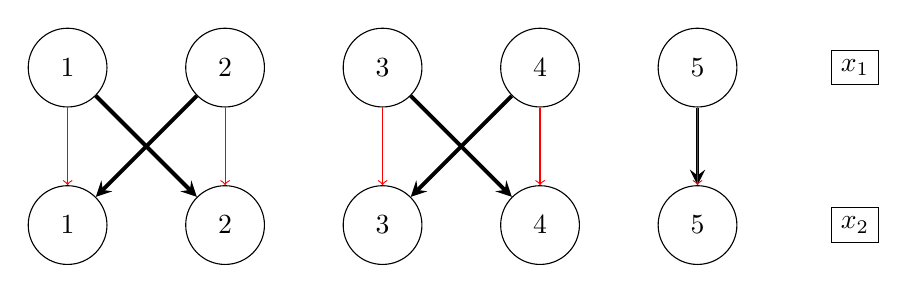
\begin{tikzpicture}[node distance=2cm, auto]
\node  (1)[draw, circle, minimum size=1cm]  {1};
\node  (2)[draw, circle, minimum size=1cm] [  right   of = 1] {2};
\node  (3)[draw, circle, minimum size=1cm] [  right  of = 2] {3};
\node  (4)[draw, circle, minimum size=1cm] [  right  of = 3] {4};
\node  (5)[draw, circle, minimum size=1cm] [  right  of = 4] {5};
\node  (x)[draw, rectangle] [  right  of = 5] {$x_1$};
\node  (6)[draw, circle, minimum size=1cm] [  below   of = 1] {1};
\node  (7)[draw, circle, minimum size=1cm] [  below  of = 2] {2};
\node  (8)[draw, circle, minimum size=1cm] [  below  of = 3] {3};
\node  (9)[draw, circle, minimum size=1cm] [  below  of = 4] {4};
\node  (10)[draw, circle, minimum size=1cm] [  below  of = 5] {5};
\node  (x)[draw, rectangle] [  right  of = 10] {$x_2$};
\draw[arrows=-stealth, line width=0.5mm] (1) -- (7);
\draw[arrows=-stealth, line width=0.5mm] (2) -- (6);
\draw[arrows=-stealth, line width=0.5mm] (3) -- (9);
\draw[arrows=-stealth, line width=0.5mm] (4) -- (8);
\draw[arrows=-stealth, line width=0.5mm] (5) -- (10);
\draw[->, color=red] (1) -- (6);
\draw[->, color=red] (2) -- (7);
\draw[->, color=red] (3) -- (8);
\draw[->, color=red] (4) -- (9);
\draw[->, color=red] (5) -- (10);
\end{tikzpicture}
\[
  e_1  = 
  \begin{pmatrix}
    1 & 2 & 3 & 4 & 5 \\
    1 & 2 & 3 & 4 & 5 
  \end{pmatrix} = id
\]}


\only<9>{
Die Permutation zwischen dem zweiten und dritten Level:\\[4pt]
\begin{tikzpicture}[node distance=2cm, auto]
\node  (6)[draw, circle, minimum size=1cm] [  below   of = 1] {1};
\node  (7)[draw, circle, minimum size=1cm] [  below  of = 2] {2};
\node  (8)[draw, circle, minimum size=1cm] [  below  of = 3] {3};
\node  (9)[draw, circle, minimum size=1cm] [  below  of = 4] {4};
\node  (10)[draw, circle, minimum size=1cm] [  below  of = 5] {5};
\node  (x)[draw, rectangle] [  right  of = 10] {$x_2$};
\node  (11)[draw, circle, minimum size=1cm] [  below   of = 6] {1};
\node  (12)[draw, circle, minimum size=1cm] [  below  of = 7] {2};
\node  (13)[draw, circle, minimum size=1cm] [  below  of = 8] {3};
\node  (14)[draw, circle, minimum size=1cm] [  below  of = 9] {4};
\node  (15)[draw, circle, minimum size=1cm] [  below  of = 10] {5};
\draw[arrows=-stealth, line width=0.5mm] (7) -- (12);
\draw[arrows=-stealth, line width=0.5mm] (6) -- (11);
\draw[arrows=-stealth, line width=0.5mm] (8) -- (13);
\draw[arrows=-stealth, line width=0.5mm] (9) -- (14);
\draw[arrows=-stealth, line width=0.5mm] (10) -- (15);
\draw[->] (6) -- (12);
\draw[->] (7) -- (11);
\draw[->] (8) -- (14);
\draw[->] (9) -- (13);
\draw[->] (10) -- (15);
\end{tikzpicture}}



\only<10>{
Die Permutation für $1-Kanten$ zwischen dem zweiten und dritten Level:\\[4pt]
\begin{tikzpicture}[node distance=2cm, auto]
\node  (6)[draw, circle, minimum size=1cm] [  below   of = 1] {1};
\node  (7)[draw, circle, minimum size=1cm] [  below  of = 2] {2};
\node  (8)[draw, circle, minimum size=1cm] [  below  of = 3] {3};
\node  (9)[draw, circle, minimum size=1cm] [  below  of = 4] {4};
\node  (10)[draw, circle, minimum size=1cm] [  below  of = 5] {5};
\node  (x)[draw, rectangle] [  right  of = 10] {$x_2$};
\node  (11)[draw, circle, minimum size=1cm] [  below   of = 6] {1};
\node  (12)[draw, circle, minimum size=1cm] [  below  of = 7] {2};
\node  (13)[draw, circle, minimum size=1cm] [  below  of = 8] {3};
\node  (14)[draw, circle, minimum size=1cm] [  below  of = 9] {4};
\node  (15)[draw, circle, minimum size=1cm] [  below  of = 10] {5};
\draw[arrows=-stealth, line width=0.5mm, color=red] (7) -- (12);
\draw[arrows=-stealth, line width=0.5mm, color=red] (6) -- (11);
\draw[arrows=-stealth, line width=0.5mm, color=red] (8) -- (13);
\draw[arrows=-stealth, line width=0.5mm, color=red] (9) -- (14);
\draw[arrows=-stealth, line width=0.5mm, color=red] (10) -- (15);
\draw[->] (6) -- (12);
\draw[->] (7) -- (11);
\draw[->] (8) -- (14);
\draw[->] (9) -- (13);
\draw[->] (10) -- (15);
\end{tikzpicture}
\[
  \sigma_2  = 
  \begin{pmatrix}
    1 & 2 & 3 & 4 & 5 \\
    1 & 2 & 3 & 4 & 5 
  \end{pmatrix} = id
\]}



\only<11>{
Die Permutation für $0-Kanten$ zwischen dem zweiten und dritten Level:\\[4pt]
\begin{tikzpicture}[node distance=2cm, auto]
\node  (6)[draw, circle, minimum size=1cm] [  below   of = 1] {1};
\node  (7)[draw, circle, minimum size=1cm] [  below  of = 2] {2};
\node  (8)[draw, circle, minimum size=1cm] [  below  of = 3] {3};
\node  (9)[draw, circle, minimum size=1cm] [  below  of = 4] {4};
\node  (10)[draw, circle, minimum size=1cm] [  below  of = 5] {5};
\node  (x)[draw, rectangle] [  right  of = 10] {$x_2$};
\node  (11)[draw, circle, minimum size=1cm] [  below   of = 6] {1};
\node  (12)[draw, circle, minimum size=1cm] [  below  of = 7] {2};
\node  (13)[draw, circle, minimum size=1cm] [  below  of = 8] {3};
\node  (14)[draw, circle, minimum size=1cm] [  below  of = 9] {4};
\node  (15)[draw, circle, minimum size=1cm] [  below  of = 10] {5};
\draw[arrows=-stealth, line width=0.5mm] (7) -- (12);
\draw[arrows=-stealth, line width=0.5mm] (6) -- (11);
\draw[arrows=-stealth, line width=0.5mm] (8) -- (13);
\draw[arrows=-stealth, line width=0.5mm] (9) -- (14);
\draw[arrows=-stealth, line width=0.5mm] (10) -- (15);
\draw[->, color=red] (6) -- (12);
\draw[->, color=red] (7) -- (11);
\draw[->, color=red] (8) -- (14);
\draw[->, color=red] (9) -- (13);
\draw[->, color=red] (10) -- (15);
\end{tikzpicture}
\[
  e_2  = 
  \begin{pmatrix}
    1 & 2 & 3 & 4 & 5 \\
    2 & 1 & 4 & 2 & 5 
  \end{pmatrix} = (1,2)(3,4)(5)
\] }



\only<12>{
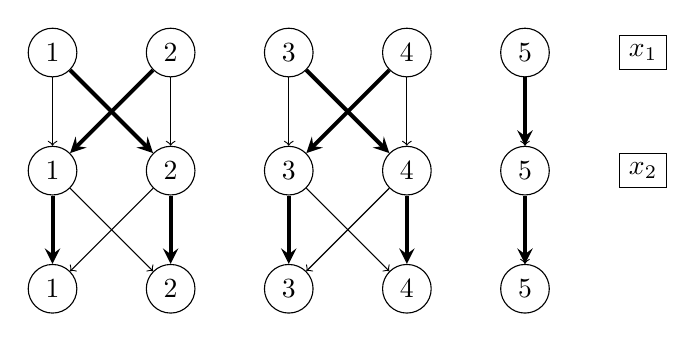
\begin{tikzpicture}[node distance=1.5cm, auto]
\node  (1)[draw, circle, minimum size=0.5cm]  {1};
\node  (2)[draw, circle, minimum size=0.5cm]   [  right   of = 1] {2};
\node  (3)[draw, circle, minimum size=0.5cm]   [  right  of = 2] {3};
\node  (4)[draw, circle, minimum size=0.5cm]   [  right  of = 3] {4};
\node  (5)[draw, circle, minimum size=0.5cm]   [  right  of = 4] {5};
\node  (x)[draw, rectangle] [  right  of = 5] {$x_1$};
\node  (6)[draw, circle, minimum size=0.5cm]   [  below   of = 1] {1};
\node  (7)[draw, circle, minimum size=0.5cm]   [  below  of = 2] {2};
\node  (8)[draw, circle, minimum size=0.5cm]   [  below  of = 3] {3};
\node  (9)[draw, circle, minimum size=0.5cm]   [  below  of = 4] {4};
\node  (10)[draw, circle, minimum size=0.5cm]   [  below  of = 5] {5};
\node  (x)[draw, rectangle] [  right  of = 10] {$x_2$};
\node  (11)[draw, circle, minimum size=0.5cm]   [  below   of = 6] {1};
\node  (12)[draw, circle, minimum size=0.5cm]   [  below  of = 7] {2};
\node  (13)[draw, circle, minimum size=0.5cm]   [  below  of = 8] {3};
\node  (14)[draw, circle, minimum size=0.5cm]   [  below  of = 9] {4};
\node  (15)[draw, circle, minimum size=0.5cm]   [  below  of = 10] {5};
\draw[arrows=-stealth, line width=0.5mm] (1) -- (7);
\draw[arrows=-stealth, line width=0.5mm] (2) -- (6);
\draw[arrows=-stealth, line width=0.5mm] (3) -- (9);
\draw[arrows=-stealth, line width=0.5mm] (4) -- (8);
\draw[arrows=-stealth, line width=0.5mm] (5) -- (10);
\draw[arrows=-stealth, line width=0.5mm] (7) -- (12);
\draw[arrows=-stealth, line width=0.5mm] (6) -- (11);
\draw[arrows=-stealth, line width=0.5mm] (8) -- (13);
\draw[arrows=-stealth, line width=0.5mm] (9) -- (14);
\draw[arrows=-stealth, line width=0.5mm] (10) -- (15);
\draw[->] (1) -- (6);
\draw[->] (2) -- (7);
\draw[->] (3) -- (8);
\draw[->] (4) -- (9);
\draw[->] (5) -- (10);
\draw[->] (6) -- (12);
\draw[->] (7) -- (11);
\draw[->] (8) -- (14);
\draw[->] (9) -- (13);
\draw[->] (10) -- (15);
\end{tikzpicture}\\[4pt] 
Bei Eingabe (0,0) $\Rightarrow$ Ausgabe = $e_1 e_2$ = $(1,2)(3,4)(5)$}


\only<13>{
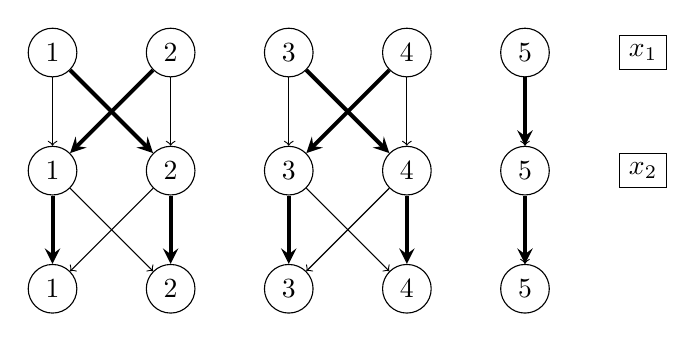
\begin{tikzpicture}[node distance=1.5cm, auto]
\node  (1)[draw, circle, minimum size=0.5cm]  {1};
\node  (2)[draw, circle, minimum size=0.5cm]   [  right   of = 1] {2};
\node  (3)[draw, circle, minimum size=0.5cm]   [  right  of = 2] {3};
\node  (4)[draw, circle, minimum size=0.5cm]   [  right  of = 3] {4};
\node  (5)[draw, circle, minimum size=0.5cm]   [  right  of = 4] {5};
\node  (x)[draw, rectangle] [  right  of = 5] {$x_1$};
\node  (6)[draw, circle, minimum size=0.5cm]   [  below   of = 1] {1};
\node  (7)[draw, circle, minimum size=0.5cm]   [  below  of = 2] {2};
\node  (8)[draw, circle, minimum size=0.5cm]   [  below  of = 3] {3};
\node  (9)[draw, circle, minimum size=0.5cm]   [  below  of = 4] {4};
\node  (10)[draw, circle, minimum size=0.5cm]   [  below  of = 5] {5};
\node  (x)[draw, rectangle] [  right  of = 10] {$x_2$};
\node  (11)[draw, circle, minimum size=0.5cm]   [  below   of = 6] {1};
\node  (12)[draw, circle, minimum size=0.5cm]   [  below  of = 7] {2};
\node  (13)[draw, circle, minimum size=0.5cm]   [  below  of = 8] {3};
\node  (14)[draw, circle, minimum size=0.5cm]   [  below  of = 9] {4};
\node  (15)[draw, circle, minimum size=0.5cm]   [  below  of = 10] {5};
\draw[arrows=-stealth, line width=0.5mm] (1) -- (7);
\draw[arrows=-stealth, line width=0.5mm] (2) -- (6);
\draw[arrows=-stealth, line width=0.5mm] (3) -- (9);
\draw[arrows=-stealth, line width=0.5mm] (4) -- (8);
\draw[arrows=-stealth, line width=0.5mm] (5) -- (10);
\draw[arrows=-stealth, line width=0.5mm] (7) -- (12);
\draw[arrows=-stealth, line width=0.5mm] (6) -- (11);
\draw[arrows=-stealth, line width=0.5mm] (8) -- (13);
\draw[arrows=-stealth, line width=0.5mm] (9) -- (14);
\draw[arrows=-stealth, line width=0.5mm] (10) -- (15);
\draw[->] (1) -- (6);
\draw[->] (2) -- (7);
\draw[->] (3) -- (8);
\draw[->] (4) -- (9);
\draw[->] (5) -- (10);
\draw[->] (6) -- (12);
\draw[->] (7) -- (11);
\draw[->] (8) -- (14);
\draw[->] (9) -- (13);
\draw[->] (10) -- (15);
\end{tikzpicture}\\[4pt]
Bei Eingabe (0,0) $\Rightarrow$ Ausgabe = $e_1 e_2$ = $(1,2)(3,4)(5)$\\[2pt]
Bei Eingabe (1,1) $\Rightarrow$ Ausgabe = $\sigma_1\sigma_2$ = $(1,2)(3,4)(5)$\\[2pt]
Bei Eingabe (0,1) $\Rightarrow$ Ausgabe = $e_1 \sigma_2$ = $id$\\[2pt]
Bei Eingabe (1,0) $\Rightarrow$ Ausgabe = $\sigma_1 e_2$ = $id$
}
\end{frame}



%%%%%%%%%%%%%%%%%%%%%%%%%%%%%%%%%%%%%%%%%%%%%%%%%%%%%%
%%%%%%%%%%%%%%%%%%%%%%%%%%%%%%%%%%%%%%%%%%%%%%%%%%%%%%
\begin{frame}{Barrington Theorem}
\begin{block}{Barrington Theorem}
Wenn eine boolesche Funktion durch DeMorgan Formel mit polynomischer Größe berechnet werden kann, dann kann sie auch durch ein 5-Branching Programm mit  polynomischer Tiefe berechnet werden.
\begin{block}{DeMorgan Formel}
\textbf{Formel}: ist ein Schaltkreis dessen Gattern höchsten \textbf{fan-out 1} haben. Die Größe von einem Formel ist die Anzahl von Gattern. \\[4pt]
\textbf{DeMorgan Schaltkreis}: ist ein Schaltkreis über die boolesche Operationen $\{\vee, \wedge\}$, aber die Eingaben sind die Variable und deren Negation.\\[4pt]
Also man kann sagen, dass eine DeMorgan Formel ein Schaltkreis mit höchsten \textbf{fan-out 1} über die boolesche Operationen $\{\vee,\lnot, \wedge\}$ ist.
\end{block} 
\end{block}
\end{frame}


%%%%%%%%%%%%%%%%%%%%%%%%%%%%%%%%%%%%%%%%%%%%%%%%%%
%%%%%%%%%%%%%%%%%%%%%%%%%%%%%%%%%%%%%%%%%%%%%%%%%%
\begin{frame}{Barrington Theorem}
\begin{block}{Satz 1}
Wenn $P$ $\sigma$-$berechnet$ $f$ und $\sigma$ eine zyklische Permutation ist, dann existiert ein Permutation-Branching-Programm $P^{'}$ mit der gleichen Größe wie $P$, welches $\tau$-$berechnet$ $f$ für eine zyklische Permutation $\tau$ .
\end{block}
\textbf{Beweis}: sei $P(x) = \sigma = \sigma_1\sigma_2\dots\sigma_t$. \\[4pt]
\begin{itemize}
\item  $\sigma$ und $\tau$ sind beide zyklische Permutationen.\\[4pt]
\item dann gilt $\tau$ = $\theta\sigma\theta^{-1}$ für beliebig Permutation $\theta$.\\[4pt]
\item dann nimm $P^{'}(x) = \theta\sigma_1\sigma_2\dots\sigma_t\theta^{-1} = \theta\sigma\theta^{-1} = \tau$, indem $\sigma_1$ durch $\theta\sigma_1$ und $\sigma_t$ durch $\sigma_t\theta^{-1}$ ersetzt werden.
\end{itemize}

\end{frame}

%%%%%%%%%%%%%%%%%%%%%%%%%%%%%%%%%%%%%%%%%%%%%%%%
%%%%%%%%%%%%%%%%%%%%%%%%%%%%%%%%%%%%%%%%%%%%%%%%
\begin{frame}{Satz 1}
\only<1>{
Sei nun $P$ durch die folgende Graph gegeben:\\[7pt]
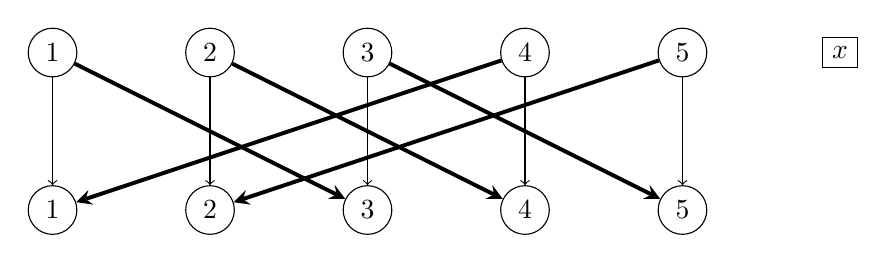
\begin{tikzpicture}[node distance=2cm, auto]
\node  (1)[draw, circle, minimum size=0.5cm]  {1};
\node  (2)[draw, circle, minimum size=0.5cm]   [  right   of = 1] {2};
\node  (3)[draw, circle, minimum size=0.5cm]   [  right  of = 2] {3};
\node  (4)[draw, circle, minimum size=0.5cm]   [  right  of = 3] {4};
\node  (5)[draw, circle, minimum size=0.5cm]   [  right  of = 4] {5};
\node  (x)[draw, rectangle] [  right  of = 5] {$x$};
\node  (6)[draw, circle, minimum size=0.5cm]  [  below  of = 1]{1};
\node  (7)[draw, circle, minimum size=0.5cm]  [  below  of = 2] {2};
\node  (8)[draw, circle, minimum size=0.5cm]  [  below  of = 3] {3};
\node  (9)[draw, circle, minimum size=0.5cm]  [  below  of = 4] {4};
\node  (10)[draw, circle, minimum size=0.5cm] [  below  of = 5] {5};
\draw[arrows=-stealth, line width=0.5mm] (1) -- (8);
\draw[arrows=-stealth, line width=0.5mm] (2) -- (9);
\draw[arrows=-stealth, line width=0.5mm] (3) -- (10);
\draw[arrows=-stealth, line width=0.5mm] (4) -- (6);
\draw[arrows=-stealth, line width=0.5mm] (5) -- (7);
\draw[->] (1) -- (6);
\draw[->] (2) -- (7);
\draw[->] (3) -- (8);
\draw[->] (4) -- (9);
\draw[->] (5) -- (10);
\end{tikzpicture}}
 
\only<2>{
Sei nun $P$ durch die folgende Graph gegeben:\\[4pt]
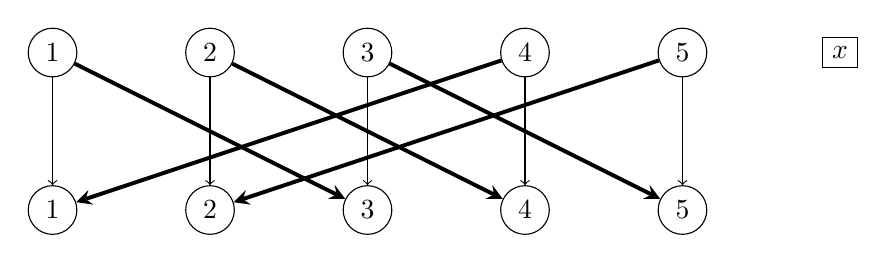
\begin{tikzpicture}[node distance=2cm, auto]
\node  (1)[draw, circle, minimum size=0.5cm]  {1};
\node  (2)[draw, circle, minimum size=0.5cm]   [  right   of = 1] {2};
\node  (3)[draw, circle, minimum size=0.5cm]   [  right  of = 2] {3};
\node  (4)[draw, circle, minimum size=0.5cm]   [  right  of = 3] {4};
\node  (5)[draw, circle, minimum size=0.5cm]   [  right  of = 4] {5};
\node  (x)[draw, rectangle] [  right  of = 5] {$x$};
\node  (6)[draw, circle, minimum size=0.5cm]  [  below  of = 1]{1};
\node  (7)[draw, circle, minimum size=0.5cm]  [  below  of = 2] {2};
\node  (8)[draw, circle, minimum size=0.5cm]  [  below  of = 3] {3};
\node  (9)[draw, circle, minimum size=0.5cm]  [  below  of = 4] {4};
\node  (10)[draw, circle, minimum size=0.5cm] [  below  of = 5] {5};
\draw[arrows=-stealth, line width=0.5mm] (1) -- (8);
\draw[arrows=-stealth, line width=0.5mm] (2) -- (9);
\draw[arrows=-stealth, line width=0.5mm] (3) -- (10);
\draw[arrows=-stealth, line width=0.5mm] (4) -- (6);
\draw[arrows=-stealth, line width=0.5mm] (5) -- (7);
\draw[->] (1) -- (6);
\draw[->] (2) -- (7);
\draw[->] (3) -- (8);
\draw[->] (4) -- (9);
\draw[->] (5) -- (10);
\end{tikzpicture}
Die 1-Kanten realisieren die Permutation $\sigma_1$ = $(1,3,5,2,4)$.\\[4pt]
Die 0-Kanten realisieren die Permutation $ \sigma_0$ = $id$. }

\only<3>{
Sei nun $P$ durch die folgende Graph gegeben:\\[4pt]
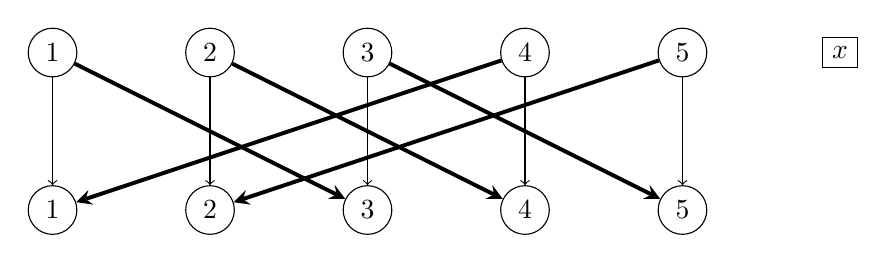
\begin{tikzpicture}[node distance=2cm, auto]
\node  (1)[draw, circle, minimum size=0.5cm]  {1};
\node  (2)[draw, circle, minimum size=0.5cm]   [  right   of = 1] {2};
\node  (3)[draw, circle, minimum size=0.5cm]   [  right  of = 2] {3};
\node  (4)[draw, circle, minimum size=0.5cm]   [  right  of = 3] {4};
\node  (5)[draw, circle, minimum size=0.5cm]   [  right  of = 4] {5};
\node  (x)[draw, rectangle] [  right  of = 5] {$x$};
\node  (6)[draw, circle, minimum size=0.5cm]  [  below  of = 1]{1};
\node  (7)[draw, circle, minimum size=0.5cm]  [  below  of = 2] {2};
\node  (8)[draw, circle, minimum size=0.5cm]  [  below  of = 3] {3};
\node  (9)[draw, circle, minimum size=0.5cm]  [  below  of = 4] {4};
\node  (10)[draw, circle, minimum size=0.5cm] [  below  of = 5] {5};
\draw[arrows=-stealth, line width=0.5mm] (1) -- (8);
\draw[arrows=-stealth, line width=0.5mm] (2) -- (9);
\draw[arrows=-stealth, line width=0.5mm] (3) -- (10);
\draw[arrows=-stealth, line width=0.5mm] (4) -- (6);
\draw[arrows=-stealth, line width=0.5mm] (5) -- (7);
\draw[->] (1) -- (6);
\draw[->] (2) -- (7);
\draw[->] (3) -- (8);
\draw[->] (4) -- (9);
\draw[->] (5) -- (10);
\end{tikzpicture}
Die 1-Kanten realisieren die Permutation $\sigma_1$ = $(1,3,5,2,4)$.\\[4pt]
Die 0-Kanten realisieren die Permutation $ \sigma_0$ = $id$. \\[4pt]
$\Rightarrow$ die berechnete Funktion ist $f(x)=$ $x$ mit $\sigma$ = $(1,3,5,2,4)$.}

\only<4>{
Sei jetzt \[
  \theta  = 
  \begin{pmatrix}
    1 & 2 & 3 & 4 & 5 \\
    3 & 4 & 1 & 5 & 2 
  \end{pmatrix} \Rightarrow \theta^{-1} = \begin{pmatrix}
    1 & 2 & 3 & 4 & 5 \\
    3 & 5 & 1 & 2 & 4 
  \end{pmatrix}.
\]}

\only<5>{
Sei jetzt \[
  \theta  = 
  \begin{pmatrix}
    1 & 2 & 3 & 4 & 5 \\
    3 & 4 & 1 & 5 & 2 
  \end{pmatrix} \Rightarrow \theta^{-1} = \begin{pmatrix}
    1 & 2 & 3 & 4 & 5 \\
    3 & 5 & 1 & 2 & 4 
  \end{pmatrix}.
\]
Jetzt berechnen wir $\theta\sigma_0\theta^{-1}$ und $\theta\sigma_1\theta^{-1}$.\\[4pt]
$\theta\sigma_0\theta^{-1} =$ $(1,3)(2,4,5)\circ id \circ (1,3)(2,5,4) =$ $id$.\\[4pt]}

\only<6>{
Sei jetzt \[
  \theta  = 
  \begin{pmatrix}
    1 & 2 & 3 & 4 & 5 \\
    3 & 4 & 1 & 5 & 2 
  \end{pmatrix} \Rightarrow \theta^{-1} = \begin{pmatrix}
    1 & 2 & 3 & 4 & 5 \\
    3 & 5 & 1 & 2 & 4 
  \end{pmatrix}.
\]
Jetzt berechnen wir $\theta\sigma_0\theta^{-1}$ und $\theta\sigma_1\theta^{-1}$.\\[4pt]
$\theta\sigma_0\theta^{-1} =$ $(1,3)(2,4,5)\circ id \circ (1,3)(2,5,4) =$ $id$.\\[4pt]
$\theta\sigma_1\theta^{-1} =$ $(1,3)(2,4,5)\circ (1,3,5,2,4) \circ (1,3)(2,5,4) =$ $(1,4,5,2,3)$.}

\only<7>{
Und somit sieht das Graph wie folgt aus:\\[4pt]
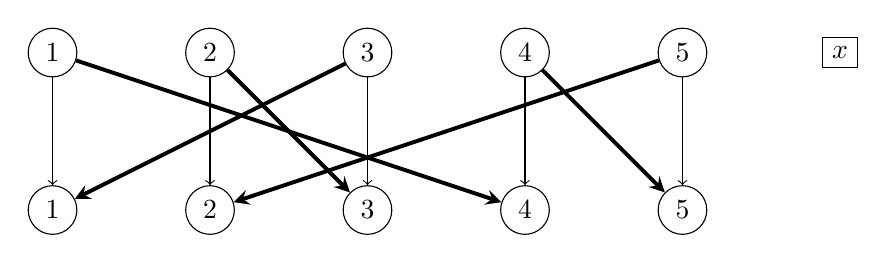
\begin{tikzpicture}[node distance=2cm, auto]
\node  (1)[draw, circle, minimum size=0.5cm]  {1};
\node  (2)[draw, circle, minimum size=0.5cm]   [  right   of = 1] {2};
\node  (3)[draw, circle, minimum size=0.5cm]   [  right  of = 2] {3};
\node  (4)[draw, circle, minimum size=0.5cm]   [  right  of = 3] {4};
\node  (5)[draw, circle, minimum size=0.5cm]   [  right  of = 4] {5};
\node  (x)[draw, rectangle] [  right  of = 5] {$x$};
\node  (6)[draw, circle, minimum size=0.5cm]  [  below  of = 1]{1};
\node  (7)[draw, circle, minimum size=0.5cm]  [  below  of = 2] {2};
\node  (8)[draw, circle, minimum size=0.5cm]  [  below  of = 3] {3};
\node  (9)[draw, circle, minimum size=0.5cm]  [  below  of = 4] {4};
\node  (10)[draw, circle, minimum size=0.5cm] [  below  of = 5] {5};
\draw[arrows=-stealth, line width=0.5mm] (1) -- (9);
\draw[arrows=-stealth, line width=0.5mm] (2) -- (8);
\draw[arrows=-stealth, line width=0.5mm] (3) -- (6);
\draw[arrows=-stealth, line width=0.5mm] (4) -- (10);
\draw[arrows=-stealth, line width=0.5mm] (5) -- (7);
\draw[->] (1) -- (6);
\draw[->] (2) -- (7);
\draw[->] (3) -- (8);
\draw[->] (4) -- (9);
\draw[->] (5) -- (10);
\end{tikzpicture}
Das Programm berechnet auch die Funktion $f(x) =$ $x$ aber durch andere Permutation und zwar $\tau = (1,4,5,2,3)$.}
\end{frame}


%%%%%%%%%%%%%%%%%%%%%%%%%%%%%%%%%%%%%%%%%%%%%%%%%%%%%%%%%%%%%%%%
%%%%%%%%%%%%%%%%%%%%%%%%%%%%%%%%%%%%%%%%%%%%%%%%%%%%%%%%%%%%%%%%
\begin{frame}{Barrington Theorem}
\begin{block}{Satz 2 (Negation)}
Wenn $P$ $\sigma$-$berechnet$ $f$ und $\sigma$ eine zyklische Permutation ist, dann existiert ein Permutation-Branching-Programm mit der selben Größe von $P$, welches $\sigma$-$berechnet$ $\lnot f$.
\end{block}
\textbf{Beweis}: Nach dem Satz 1 können wir ein PBP $P^{'}$ kriegen, welches $\sigma^{-1}$-berechnet $f$.
\begin{itemize}
\item rechne $P^{'}(x) = \sigma^{-1} = \sigma_1\sigma_2\dots\sigma_t$, $\sigma^{-1}$-berechnet $f$ mit Satz-1.
\item dann gilt: $P^{'}(x)$ = $\sigma^{-1}$ falls $f(x)$ = 1, und $P^{'}(x)$ = $e$ falls $f(x)$ = 0.
\item nimm $P^{''}(x) = \sigma_1\sigma_2\dots\sigma_t\sigma$, indem $\sigma_t$ durch $\sigma_t\sigma$ ersetzt wird. 
\end{itemize} 


\end{frame}


\begin{frame}
\only<1>{
Angewendet auf Beispiel von Satz 1:\\[4pt]
\[
  \sigma  = 
  \begin{pmatrix}
    1 & 2 & 3 & 4 & 5 \\
    3 & 4 & 5 & 1 & 2 
  \end{pmatrix} \Rightarrow \sigma^{-1}  = 
  \begin{pmatrix}
    1 & 2 & 3 & 4 & 5 \\
    4 & 5 & 1 & 2 & 3 
  \end{pmatrix}.
\]
}

\only<2>{
Angewendet auf Beispiel von Satz 1:\\[4pt]
\[
  \sigma  = 
  \begin{pmatrix}
    1 & 2 & 3 & 4 & 5 \\
    3 & 4 & 5 & 1 & 2 
  \end{pmatrix} \Rightarrow \sigma^{-1}  = 
  \begin{pmatrix}
    1 & 2 & 3 & 4 & 5 \\
    4 & 5 & 1 & 2 & 3 
  \end{pmatrix}.
\]
Die neue Permutation für die 1-Kanten ist: \\[4pt]
$\sigma^{-1}\sigma =$ $id$.\\[4pt]
Die neue Permutation für die 0-Kanten ist: \\[4pt]
$\sigma^{-1} id=$ $\sigma^{-1} =$ $(1,4,2,5,3)$.\\[4pt]
}

\only<3>{
Und somit sieht das Graph wie folgt aus:\\[4pt]
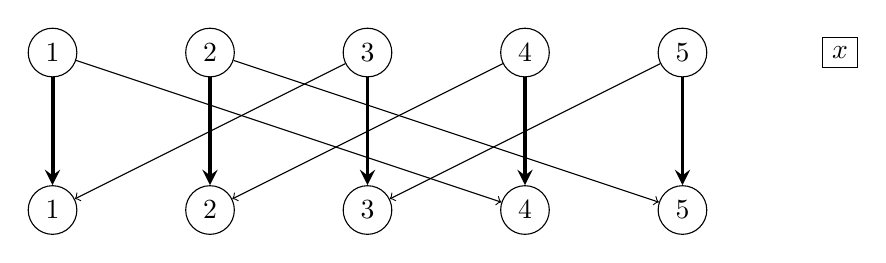
\begin{tikzpicture}[node distance=2cm, auto]
\node  (1)[draw, circle, minimum size=0.5cm]  {1};
\node  (2)[draw, circle, minimum size=0.5cm]   [  right   of = 1] {2};
\node  (3)[draw, circle, minimum size=0.5cm]   [  right  of = 2] {3};
\node  (4)[draw, circle, minimum size=0.5cm]   [  right  of = 3] {4};
\node  (5)[draw, circle, minimum size=0.5cm]   [  right  of = 4] {5};
\node  (x)[draw, rectangle] [  right  of = 5] {$x$};
\node  (6)[draw, circle, minimum size=0.5cm]  [  below  of = 1]{1};
\node  (7)[draw, circle, minimum size=0.5cm]  [  below  of = 2] {2};
\node  (8)[draw, circle, minimum size=0.5cm]  [  below  of = 3] {3};
\node  (9)[draw, circle, minimum size=0.5cm]  [  below  of = 4] {4};
\node  (10)[draw, circle, minimum size=0.5cm] [  below  of = 5] {5};
\draw[arrows=-stealth, line width=0.5mm] (1) -- (6);
\draw[arrows=-stealth, line width=0.5mm] (2) -- (7);
\draw[arrows=-stealth, line width=0.5mm] (3) -- (8);
\draw[arrows=-stealth, line width=0.5mm] (4) -- (9);
\draw[arrows=-stealth, line width=0.5mm] (5) -- (10);
\draw[->] (1) -- (9);
\draw[->] (2) -- (10);
\draw[->] (3) -- (6);
\draw[->] (4) -- (7);
\draw[->] (5) -- (8);
\end{tikzpicture}
Das Programm berechnet die Funktion $\lnot f(x)=$ $x$.
}
\end{frame}






%%%%%%%%%%%%%%%%%%%%%%%%%%%%%%%%%%%%%%%%%%%%%%%%%%%%%%
%%%%%%%%%%%%%%%%%%%%%%%%%%%%%%%%%%%%%%%%%%%%%%%%%%%%%%
\begin{frame}{Barrington Theorem}
\begin{block}{Satz 3 (AND)}
Wenn $P$ $\sigma$-$berechnet$ $f$ und $Q$ $\tau$-$berechnet$ $g$, dann existiert ein PBP mit der Tiefe 2($\mid$$P$$\mid$ + $\mid$$Q$$\mid$), welches \\[2pt]
$\sigma\tau\sigma^{-1}\tau^{-1}$-$berechnet$ $f$ $\wedge$ $g$.
\end{block}
$Beweis$: Nach dem Satz 1 bekommen wir ein Programm mit $\sigma^{-1}$-$berechnet$ $f$ und das andere mit $\tau^{-1}$-$berechnet$ $g$.\\[4pt]
Wir komponieren die 4 Programme in diese Reihenfolge $\sigma^{'}$ = $\sigma\tau\sigma^{-1}\tau^{-1}$. Wenn  $f$ = 0 und $g$ = 0, dann ist $\sigma^{'}$ = id$\circ$id$\circ$id$\circ$id = id. 
Für den Fall $f$ = 1 und $g$ = 1 brauchen wir den Folgenden Satz.\\[4pt]
\begin{block}{Satz 4}
Es gibt zwei zyklische Permutationen auf [5] $\sigma$ und $\tau$ so, dass
  $\sigma \tau \sigma^{-1} \tau^{-1}$ zyklisch ist.
\\[4pt]
$Beweis$: Durch ein Beispiel. 
\end{block}
\end{frame}




%%%%%%%%%%%%%%%%%%%%%%%%%%%%%%%%%%%%%%%%%%%%%%%%%%%%%%%%%%%%%%%%
%%%%%%%%%%%%%%%%%%%%%%%%%%%%%%%%%%%%%%%%%%%%%%%%%%%%%%%%%%%%%%%%
\begin{frame}{Barrington Theorem}

\only<1>{
\[ \sigma  = 
  \begin{pmatrix}
    1 & 2 & 3 & 4 & 5 \\
    2 & 3 & 4 & 5 & 1 
  \end{pmatrix} , \tau  = 
  \begin{pmatrix}
    1 & 2 & 3 & 4 & 5 \\
    3 & 1 & 5 & 2 & 4 
  \end{pmatrix}
\]
}

\only<2>{
\[ \sigma  = 
  \begin{pmatrix}
    1 & 2 & 3 & 4 & 5 \\
    2 & 3 & 4 & 5 & 1 
  \end{pmatrix} , \tau  = 
  \begin{pmatrix}
    1 & 2 & 3 & 4 & 5 \\
    3 & 1 & 5 & 2 & 4 
  \end{pmatrix}
\]
\[ \sigma^{-1}  = 
  \begin{pmatrix}
    1 & 2 & 3 & 4 & 5 \\
    5 & 1 & 2 & 3 & 4 
  \end{pmatrix} , \tau^{-1}  = 
  \begin{pmatrix}
    1 & 2 & 3 & 4 & 5 \\
    2 & 4 & 1 & 5 & 3 
  \end{pmatrix}
\]
}

\only<3>{
\[ \sigma  = 
  \begin{pmatrix}
    1 & 2 & 3 & 4 & 5 \\
    2 & 3 & 4 & 5 & 1 
  \end{pmatrix} , \tau  = 
  \begin{pmatrix}
    1 & 2 & 3 & 4 & 5 \\
    3 & 1 & 5 & 2 & 4 
  \end{pmatrix}
\]
\[ \sigma^{-1}  = 
  \begin{pmatrix}
    1 & 2 & 3 & 4 & 5 \\
    5 & 1 & 2 & 3 & 4 
  \end{pmatrix} , \tau^{-1}  = 
  \begin{pmatrix}
    1 & 2 & 3 & 4 & 5 \\
    2 & 4 & 1 & 5 & 3 
  \end{pmatrix}
\]
\[ \sigma\tau\sigma^{-1}\tau^{-1}  = 
  \begin{pmatrix}
    1 & 2 & 3 & 4 & 5 \\
    3 & 5 & 2 & 1 & 4 
  \end{pmatrix} 
\]
}


\only<4>{
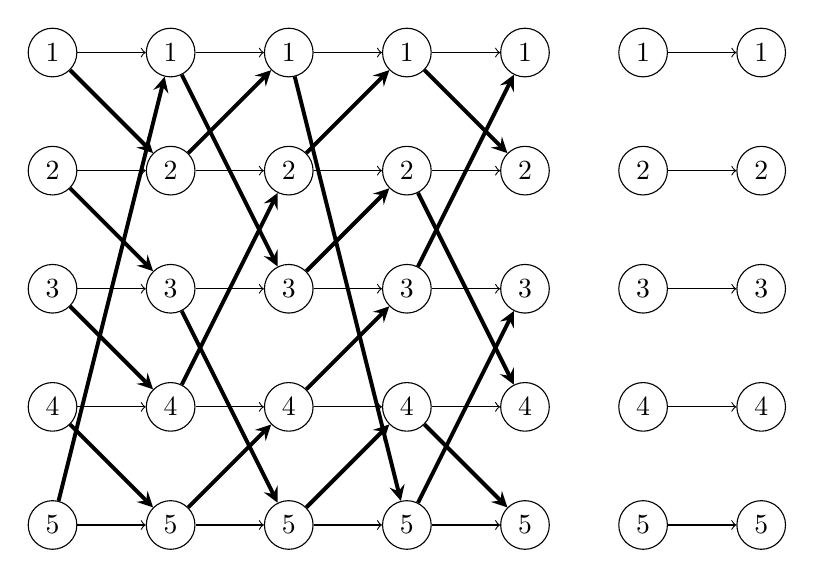
\begin{tikzpicture}[node distance=1.5cm, auto]
\node  (1)[draw, circle, minimum size=0.5cm]  {1};
\node  (2)[draw, circle, minimum size=0.5cm] [  below   of = 1] {2};
\node  (3)[draw, circle, minimum size=0.5cm] [  below  of = 2] {3};
\node  (4)[draw, circle, minimum size=0.5cm] [  below  of = 3] {4};
\node  (5)[draw, circle, minimum size=0.5cm] [  below  of = 4] {5};
\node  (6)[draw, circle, minimum size=0.5cm] [  right   of = 1] {1};
\node  (7)[draw, circle, minimum size=0.5cm] [  right  of = 2] {2};
\node  (8)[draw, circle, minimum size=0.5cm] [  right  of = 3] {3};
\node  (9)[draw, circle, minimum size=0.5cm] [  right  of = 4] {4};
\node  (10)[draw, circle, minimum size=0.5cm] [  right  of = 5] {5};
\node  (11)[draw, circle, minimum size=0.5cm] [  right   of = 6] {1};
\node  (12)[draw, circle, minimum size=0.5cm] [  right  of = 7] {2};
\node  (13)[draw, circle, minimum size=0.5cm] [  right  of = 8] {3};
\node  (14)[draw, circle, minimum size=0.5cm] [  right  of = 9] {4};
\node  (15)[draw, circle, minimum size=0.5cm] [  right  of = 10] {5};
\node  (16)[draw, circle, minimum size=0.5cm] [  right   of = 11] {1};
\node  (17)[draw, circle, minimum size=0.5cm] [  right  of = 12] {2};
\node  (18)[draw, circle, minimum size=0.5cm] [  right  of = 13] {3};
\node  (19)[draw, circle, minimum size=0.5cm] [  right  of = 14] {4};
\node  (20)[draw, circle, minimum size=0.5cm] [  right  of = 15] {5};
\node  (21)[draw, circle, minimum size=0.5cm] [  right   of = 16] {1};
\node  (22)[draw, circle, minimum size=0.5cm] [  right  of = 17] {2};
\node  (23)[draw, circle, minimum size=0.5cm] [  right  of = 18] {3};
\node  (24)[draw, circle, minimum size=0.5cm] [  right  of = 19] {4};
\node  (25)[draw, circle, minimum size=0.5cm] [  right  of = 20] {5};
\node  (26)[draw, circle, minimum size=0.5cm] [  right   of = 21] {1};
\node  (27)[draw, circle, minimum size=0.5cm] [  right  of = 22] {2};
\node  (28)[draw, circle, minimum size=0.5cm] [  right  of = 23] {3};
\node  (29)[draw, circle, minimum size=0.5cm] [  right  of = 24] {4};
\node  (30)[draw, circle, minimum size=0.5cm] [  right  of = 25] {5};
\node  (31)[draw, circle, minimum size=0.5cm] [  right   of = 26] {1};
\node  (32)[draw, circle, minimum size=0.5cm] [  right  of = 27] {2};
\node  (33)[draw, circle, minimum size=0.5cm] [  right  of = 28] {3};
\node  (34)[draw, circle, minimum size=0.5cm] [  right  of = 29] {4};
\node  (35)[draw, circle, minimum size=0.5cm] [  right  of = 30] {5};
\draw[arrows=-stealth, line width=0.5mm] (1) -- (7);
\draw[arrows=-stealth, line width=0.5mm] (2) -- (8);
\draw[arrows=-stealth, line width=0.5mm] (3) -- (9);
\draw[arrows=-stealth, line width=0.5mm] (4) -- (10);
\draw[arrows=-stealth, line width=0.5mm] (5) -- (6);
\draw[arrows=-stealth, line width=0.5mm] (6) -- (13);
\draw[arrows=-stealth, line width=0.5mm] (7) -- (11);
\draw[arrows=-stealth, line width=0.5mm] (8) -- (15);
\draw[arrows=-stealth, line width=0.5mm] (9) -- (12);
\draw[arrows=-stealth, line width=0.5mm] (10) -- (14);
\draw[arrows=-stealth, line width=0.5mm] (11) -- (20);
\draw[arrows=-stealth, line width=0.5mm] (12) -- (16);
\draw[arrows=-stealth, line width=0.5mm] (13) -- (17);
\draw[arrows=-stealth, line width=0.5mm] (14) -- (18);
\draw[arrows=-stealth, line width=0.5mm] (15) -- (19);
\draw[arrows=-stealth, line width=0.5mm] (16) -- (22);
\draw[arrows=-stealth, line width=0.5mm] (17) -- (24);
\draw[arrows=-stealth, line width=0.5mm] (18) -- (21);
\draw[arrows=-stealth, line width=0.5mm] (19) -- (25);
\draw[arrows=-stealth, line width=0.5mm] (20) -- (23);
\draw[->] (1) -- (6);
\draw[->] (2) -- (7);
\draw[->] (3) -- (8);
\draw[->] (4) -- (9);
\draw[->] (5) -- (10);
\draw[->] (6) -- (11);
\draw[->] (7) -- (12);
\draw[->] (8) -- (13);
\draw[->] (9) -- (14);
\draw[->] (10) -- (15);
\draw[->] (11) -- (16);
\draw[->] (12) -- (17);
\draw[->] (13) -- (18);
\draw[->] (14) -- (19);
\draw[->] (15) -- (20);
\draw[->] (16) -- (21);
\draw[->] (17) -- (22);
\draw[->] (18) -- (23);
\draw[->] (19) -- (24);
\draw[->] (20) -- (25);
\draw[->] (26) -- (31);
\draw[->] (27) -- (32);
\draw[->] (28) -- (33);
\draw[->] (29) -- (34);
\draw[->] (30) -- (35);
\end{tikzpicture}}


\only<5>{
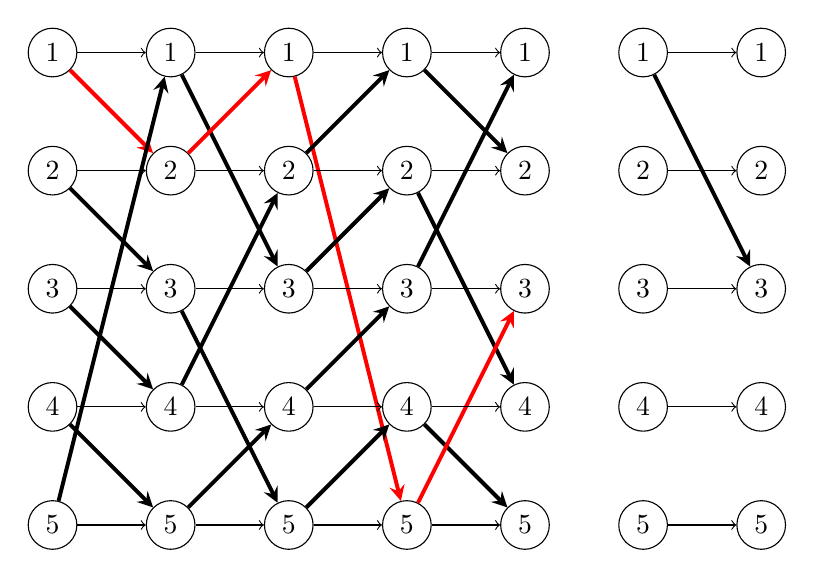
\begin{tikzpicture}[node distance=1.5cm, auto]
\node  (1)[draw, circle, minimum size=0.5cm]  {1};
\node  (2)[draw, circle, minimum size=0.5cm] [  below   of = 1] {2};
\node  (3)[draw, circle, minimum size=0.5cm] [  below  of = 2] {3};
\node  (4)[draw, circle, minimum size=0.5cm] [  below  of = 3] {4};
\node  (5)[draw, circle, minimum size=0.5cm] [  below  of = 4] {5};
\node  (6)[draw, circle, minimum size=0.5cm] [  right   of = 1] {1};
\node  (7)[draw, circle, minimum size=0.5cm] [  right  of = 2] {2};
\node  (8)[draw, circle, minimum size=0.5cm] [  right  of = 3] {3};
\node  (9)[draw, circle, minimum size=0.5cm] [  right  of = 4] {4};
\node  (10)[draw, circle, minimum size=0.5cm] [  right  of = 5] {5};
\node  (11)[draw, circle, minimum size=0.5cm] [  right   of = 6] {1};
\node  (12)[draw, circle, minimum size=0.5cm] [  right  of = 7] {2};
\node  (13)[draw, circle, minimum size=0.5cm] [  right  of = 8] {3};
\node  (14)[draw, circle, minimum size=0.5cm] [  right  of = 9] {4};
\node  (15)[draw, circle, minimum size=0.5cm] [  right  of = 10] {5};
\node  (16)[draw, circle, minimum size=0.5cm] [  right   of = 11] {1};
\node  (17)[draw, circle, minimum size=0.5cm] [  right  of = 12] {2};
\node  (18)[draw, circle, minimum size=0.5cm] [  right  of = 13] {3};
\node  (19)[draw, circle, minimum size=0.5cm] [  right  of = 14] {4};
\node  (20)[draw, circle, minimum size=0.5cm] [  right  of = 15] {5};
\node  (21)[draw, circle, minimum size=0.5cm] [  right   of = 16] {1};
\node  (22)[draw, circle, minimum size=0.5cm] [  right  of = 17] {2};
\node  (23)[draw, circle, minimum size=0.5cm] [  right  of = 18] {3};
\node  (24)[draw, circle, minimum size=0.5cm] [  right  of = 19] {4};
\node  (25)[draw, circle, minimum size=0.5cm] [  right  of = 20] {5};
\node  (26)[draw, circle, minimum size=0.5cm] [  right   of = 21] {1};
\node  (27)[draw, circle, minimum size=0.5cm] [  right  of = 22] {2};
\node  (28)[draw, circle, minimum size=0.5cm] [  right  of = 23] {3};
\node  (29)[draw, circle, minimum size=0.5cm] [  right  of = 24] {4};
\node  (30)[draw, circle, minimum size=0.5cm] [  right  of = 25] {5};
\node  (31)[draw, circle, minimum size=0.5cm] [  right   of = 26] {1};
\node  (32)[draw, circle, minimum size=0.5cm] [  right  of = 27] {2};
\node  (33)[draw, circle, minimum size=0.5cm] [  right  of = 28] {3};
\node  (34)[draw, circle, minimum size=0.5cm] [  right  of = 29] {4};
\node  (35)[draw, circle, minimum size=0.5cm] [  right  of = 30] {5};
\draw[arrows=-stealth, line width=0.5mm, color=red] (1) -- (7);
\draw[arrows=-stealth, line width=0.5mm] (2) -- (8);
\draw[arrows=-stealth, line width=0.5mm] (3) -- (9);
\draw[arrows=-stealth, line width=0.5mm] (4) -- (10);
\draw[arrows=-stealth, line width=0.5mm] (5) -- (6);
\draw[arrows=-stealth, line width=0.5mm] (6) -- (13);
\draw[arrows=-stealth, line width=0.5mm, color=red] (7) -- (11);
\draw[arrows=-stealth, line width=0.5mm] (8) -- (15);
\draw[arrows=-stealth, line width=0.5mm] (9) -- (12);
\draw[arrows=-stealth, line width=0.5mm] (10) -- (14);
\draw[arrows=-stealth, line width=0.5mm, color=red] (11) -- (20);
\draw[arrows=-stealth, line width=0.5mm] (12) -- (16);
\draw[arrows=-stealth, line width=0.5mm] (13) -- (17);
\draw[arrows=-stealth, line width=0.5mm] (14) -- (18);
\draw[arrows=-stealth, line width=0.5mm] (15) -- (19);
\draw[arrows=-stealth, line width=0.5mm] (16) -- (22);
\draw[arrows=-stealth, line width=0.5mm] (17) -- (24);
\draw[arrows=-stealth, line width=0.5mm] (18) -- (21);
\draw[arrows=-stealth, line width=0.5mm] (19) -- (25);
\draw[arrows=-stealth, line width=0.5mm, color=red] (20) -- (23);
\draw[arrows=-stealth, line width=0.5mm] (26) -- (33);
\draw[->] (1) -- (6);
\draw[->] (2) -- (7);
\draw[->] (3) -- (8);
\draw[->] (4) -- (9);
\draw[->] (5) -- (10);
\draw[->] (6) -- (11);
\draw[->] (7) -- (12);
\draw[->] (8) -- (13);
\draw[->] (9) -- (14);
\draw[->] (10) -- (15);
\draw[->] (11) -- (16);
\draw[->] (12) -- (17);
\draw[->] (13) -- (18);
\draw[->] (14) -- (19);
\draw[->] (15) -- (20);
\draw[->] (16) -- (21);
\draw[->] (17) -- (22);
\draw[->] (18) -- (23);
\draw[->] (19) -- (24);
\draw[->] (20) -- (25);
\draw[->] (26) -- (31);
\draw[->] (27) -- (32);
\draw[->] (28) -- (33);
\draw[->] (29) -- (34);
\draw[->] (30) -- (35);
\end{tikzpicture}
}

\only<6>{
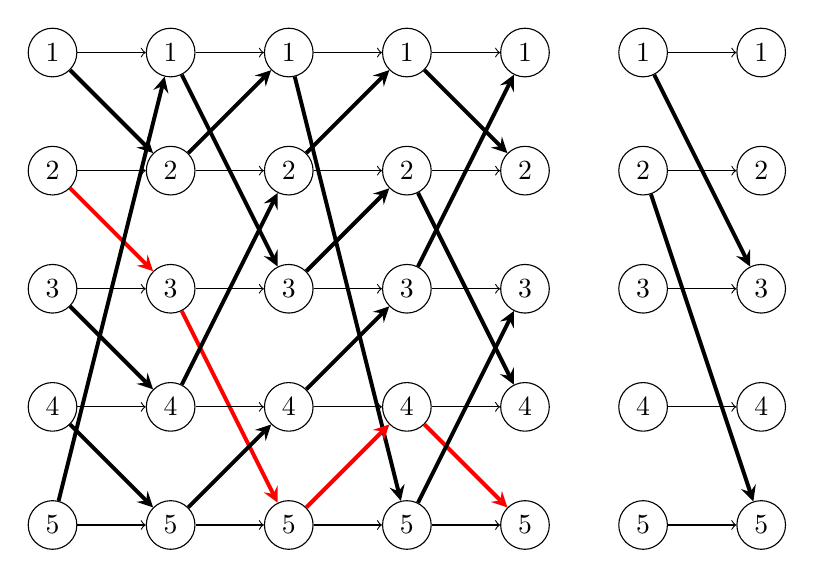
\begin{tikzpicture}[node distance=1.5cm, auto]
\node  (1)[draw, circle, minimum size=0.5cm]  {1};
\node  (2)[draw, circle, minimum size=0.5cm] [  below   of = 1] {2};
\node  (3)[draw, circle, minimum size=0.5cm] [  below  of = 2] {3};
\node  (4)[draw, circle, minimum size=0.5cm] [  below  of = 3] {4};
\node  (5)[draw, circle, minimum size=0.5cm] [  below  of = 4] {5};
\node  (6)[draw, circle, minimum size=0.5cm] [  right   of = 1] {1};
\node  (7)[draw, circle, minimum size=0.5cm] [  right  of = 2] {2};
\node  (8)[draw, circle, minimum size=0.5cm] [  right  of = 3] {3};
\node  (9)[draw, circle, minimum size=0.5cm] [  right  of = 4] {4};
\node  (10)[draw, circle, minimum size=0.5cm] [  right  of = 5] {5};
\node  (11)[draw, circle, minimum size=0.5cm] [  right   of = 6] {1};
\node  (12)[draw, circle, minimum size=0.5cm] [  right  of = 7] {2};
\node  (13)[draw, circle, minimum size=0.5cm] [  right  of = 8] {3};
\node  (14)[draw, circle, minimum size=0.5cm] [  right  of = 9] {4};
\node  (15)[draw, circle, minimum size=0.5cm] [  right  of = 10] {5};
\node  (16)[draw, circle, minimum size=0.5cm] [  right   of = 11] {1};
\node  (17)[draw, circle, minimum size=0.5cm] [  right  of = 12] {2};
\node  (18)[draw, circle, minimum size=0.5cm] [  right  of = 13] {3};
\node  (19)[draw, circle, minimum size=0.5cm] [  right  of = 14] {4};
\node  (20)[draw, circle, minimum size=0.5cm] [  right  of = 15] {5};
\node  (21)[draw, circle, minimum size=0.5cm] [  right   of = 16] {1};
\node  (22)[draw, circle, minimum size=0.5cm] [  right  of = 17] {2};
\node  (23)[draw, circle, minimum size=0.5cm] [  right  of = 18] {3};
\node  (24)[draw, circle, minimum size=0.5cm] [  right  of = 19] {4};
\node  (25)[draw, circle, minimum size=0.5cm] [  right  of = 20] {5};
\node  (26)[draw, circle, minimum size=0.5cm] [  right   of = 21] {1};
\node  (27)[draw, circle, minimum size=0.5cm] [  right  of = 22] {2};
\node  (28)[draw, circle, minimum size=0.5cm] [  right  of = 23] {3};
\node  (29)[draw, circle, minimum size=0.5cm] [  right  of = 24] {4};
\node  (30)[draw, circle, minimum size=0.5cm] [  right  of = 25] {5};
\node  (31)[draw, circle, minimum size=0.5cm] [  right   of = 26] {1};
\node  (32)[draw, circle, minimum size=0.5cm] [  right  of = 27] {2};
\node  (33)[draw, circle, minimum size=0.5cm] [  right  of = 28] {3};
\node  (34)[draw, circle, minimum size=0.5cm] [  right  of = 29] {4};
\node  (35)[draw, circle, minimum size=0.5cm] [  right  of = 30] {5};
\draw[arrows=-stealth, line width=0.5mm] (1) -- (7);
\draw[arrows=-stealth, line width=0.5mm, color=red] (2) -- (8);
\draw[arrows=-stealth, line width=0.5mm] (3) -- (9);
\draw[arrows=-stealth, line width=0.5mm] (4) -- (10);
\draw[arrows=-stealth, line width=0.5mm] (5) -- (6);
\draw[arrows=-stealth, line width=0.5mm] (6) -- (13);
\draw[arrows=-stealth, line width=0.5mm] (7) -- (11);
\draw[arrows=-stealth, line width=0.5mm, color=red] (8) -- (15);
\draw[arrows=-stealth, line width=0.5mm] (9) -- (12);
\draw[arrows=-stealth, line width=0.5mm] (10) -- (14);
\draw[arrows=-stealth, line width=0.5mm] (11) -- (20);
\draw[arrows=-stealth, line width=0.5mm] (12) -- (16);
\draw[arrows=-stealth, line width=0.5mm] (13) -- (17);
\draw[arrows=-stealth, line width=0.5mm] (14) -- (18);
\draw[arrows=-stealth, line width=0.5mm, color=red] (15) -- (19);
\draw[arrows=-stealth, line width=0.5mm] (16) -- (22);
\draw[arrows=-stealth, line width=0.5mm] (17) -- (24);
\draw[arrows=-stealth, line width=0.5mm] (18) -- (21);
\draw[arrows=-stealth, line width=0.5mm, color=red] (19) -- (25);
\draw[arrows=-stealth, line width=0.5mm] (20) -- (23);
\draw[arrows=-stealth, line width=0.5mm] (26) -- (33);
\draw[arrows=-stealth, line width=0.5mm] (27) -- (35);
\draw[->] (1) -- (6);
\draw[->] (2) -- (7);
\draw[->] (3) -- (8);
\draw[->] (4) -- (9);
\draw[->] (5) -- (10);
\draw[->] (6) -- (11);
\draw[->] (7) -- (12);
\draw[->] (8) -- (13);
\draw[->] (9) -- (14);
\draw[->] (10) -- (15);
\draw[->] (11) -- (16);
\draw[->] (12) -- (17);
\draw[->] (13) -- (18);
\draw[->] (14) -- (19);
\draw[->] (15) -- (20);
\draw[->] (16) -- (21);
\draw[->] (17) -- (22);
\draw[->] (18) -- (23);
\draw[->] (19) -- (24);
\draw[->] (20) -- (25);
\draw[->] (26) -- (31);
\draw[->] (27) -- (32);
\draw[->] (28) -- (33);
\draw[->] (29) -- (34);
\draw[->] (30) -- (35);
\end{tikzpicture}
}

\only<7>{
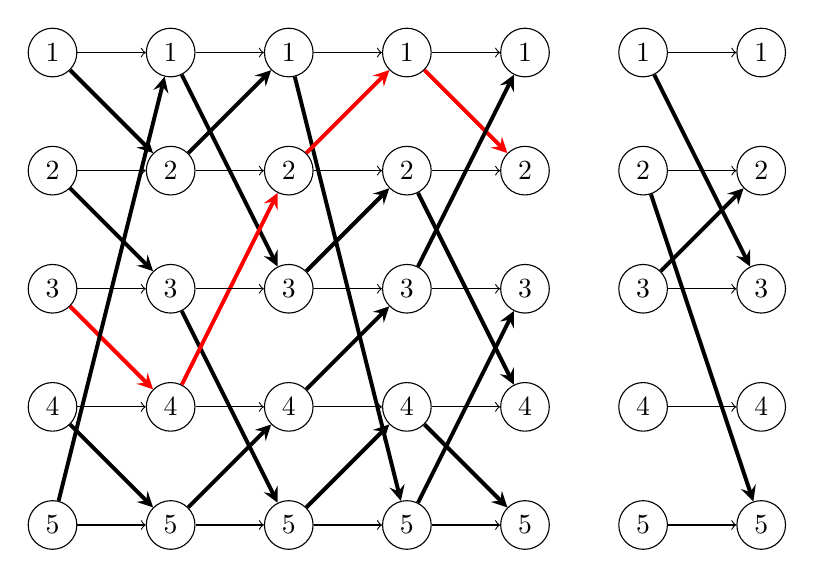
\begin{tikzpicture}[node distance=1.5cm, auto]
\node  (1)[draw, circle, minimum size=0.5cm]  {1};
\node  (2)[draw, circle, minimum size=0.5cm] [  below   of = 1] {2};
\node  (3)[draw, circle, minimum size=0.5cm] [  below  of = 2] {3};
\node  (4)[draw, circle, minimum size=0.5cm] [  below  of = 3] {4};
\node  (5)[draw, circle, minimum size=0.5cm] [  below  of = 4] {5};
\node  (6)[draw, circle, minimum size=0.5cm] [  right   of = 1] {1};
\node  (7)[draw, circle, minimum size=0.5cm] [  right  of = 2] {2};
\node  (8)[draw, circle, minimum size=0.5cm] [  right  of = 3] {3};
\node  (9)[draw, circle, minimum size=0.5cm] [  right  of = 4] {4};
\node  (10)[draw, circle, minimum size=0.5cm] [  right  of = 5] {5};
\node  (11)[draw, circle, minimum size=0.5cm] [  right   of = 6] {1};
\node  (12)[draw, circle, minimum size=0.5cm] [  right  of = 7] {2};
\node  (13)[draw, circle, minimum size=0.5cm] [  right  of = 8] {3};
\node  (14)[draw, circle, minimum size=0.5cm] [  right  of = 9] {4};
\node  (15)[draw, circle, minimum size=0.5cm] [  right  of = 10] {5};
\node  (16)[draw, circle, minimum size=0.5cm] [  right   of = 11] {1};
\node  (17)[draw, circle, minimum size=0.5cm] [  right  of = 12] {2};
\node  (18)[draw, circle, minimum size=0.5cm] [  right  of = 13] {3};
\node  (19)[draw, circle, minimum size=0.5cm] [  right  of = 14] {4};
\node  (20)[draw, circle, minimum size=0.5cm] [  right  of = 15] {5};
\node  (21)[draw, circle, minimum size=0.5cm] [  right   of = 16] {1};
\node  (22)[draw, circle, minimum size=0.5cm] [  right  of = 17] {2};
\node  (23)[draw, circle, minimum size=0.5cm] [  right  of = 18] {3};
\node  (24)[draw, circle, minimum size=0.5cm] [  right  of = 19] {4};
\node  (25)[draw, circle, minimum size=0.5cm] [  right  of = 20] {5};
\node  (26)[draw, circle, minimum size=0.5cm] [  right   of = 21] {1};
\node  (27)[draw, circle, minimum size=0.5cm] [  right  of = 22] {2};
\node  (28)[draw, circle, minimum size=0.5cm] [  right  of = 23] {3};
\node  (29)[draw, circle, minimum size=0.5cm] [  right  of = 24] {4};
\node  (30)[draw, circle, minimum size=0.5cm] [  right  of = 25] {5};
\node  (31)[draw, circle, minimum size=0.5cm] [  right   of = 26] {1};
\node  (32)[draw, circle, minimum size=0.5cm] [  right  of = 27] {2};
\node  (33)[draw, circle, minimum size=0.5cm] [  right  of = 28] {3};
\node  (34)[draw, circle, minimum size=0.5cm] [  right  of = 29] {4};
\node  (35)[draw, circle, minimum size=0.5cm] [  right  of = 30] {5};
\draw[arrows=-stealth, line width=0.5mm] (1) -- (7);
\draw[arrows=-stealth, line width=0.5mm] (2) -- (8);
\draw[arrows=-stealth, line width=0.5mm, color=red] (3) -- (9);
\draw[arrows=-stealth, line width=0.5mm] (4) -- (10);
\draw[arrows=-stealth, line width=0.5mm] (5) -- (6);
\draw[arrows=-stealth, line width=0.5mm] (6) -- (13);
\draw[arrows=-stealth, line width=0.5mm] (7) -- (11);
\draw[arrows=-stealth, line width=0.5mm] (8) -- (15);
\draw[arrows=-stealth, line width=0.5mm, color=red] (9) -- (12);
\draw[arrows=-stealth, line width=0.5mm] (10) -- (14);
\draw[arrows=-stealth, line width=0.5mm] (11) -- (20);
\draw[arrows=-stealth, line width=0.5mm, color=red] (12) -- (16);
\draw[arrows=-stealth, line width=0.5mm] (13) -- (17);
\draw[arrows=-stealth, line width=0.5mm] (14) -- (18);
\draw[arrows=-stealth, line width=0.5mm] (15) -- (19);
\draw[arrows=-stealth, line width=0.5mm, color=red] (16) -- (22);
\draw[arrows=-stealth, line width=0.5mm] (17) -- (24);
\draw[arrows=-stealth, line width=0.5mm] (18) -- (21);
\draw[arrows=-stealth, line width=0.5mm] (19) -- (25);
\draw[arrows=-stealth, line width=0.5mm] (20) -- (23);
\draw[arrows=-stealth, line width=0.5mm] (26) -- (33);
\draw[arrows=-stealth, line width=0.5mm] (27) -- (35);
\draw[arrows=-stealth, line width=0.5mm] (28) -- (32);
\draw[->] (1) -- (6);
\draw[->] (2) -- (7);
\draw[->] (3) -- (8);
\draw[->] (4) -- (9);
\draw[->] (5) -- (10);
\draw[->] (6) -- (11);
\draw[->] (7) -- (12);
\draw[->] (8) -- (13);
\draw[->] (9) -- (14);
\draw[->] (10) -- (15);
\draw[->] (11) -- (16);
\draw[->] (12) -- (17);
\draw[->] (13) -- (18);
\draw[->] (14) -- (19);
\draw[->] (15) -- (20);
\draw[->] (16) -- (21);
\draw[->] (17) -- (22);
\draw[->] (18) -- (23);
\draw[->] (19) -- (24);
\draw[->] (20) -- (25);
\draw[->] (26) -- (31);
\draw[->] (27) -- (32);
\draw[->] (28) -- (33);
\draw[->] (29) -- (34);
\draw[->] (30) -- (35);
\end{tikzpicture}
}


\only<8>{
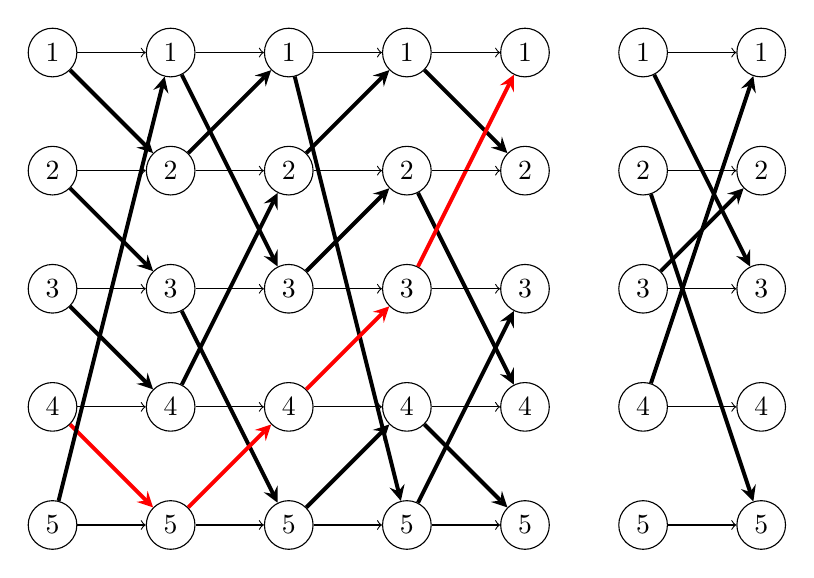
\begin{tikzpicture}[node distance=1.5cm, auto]
\node  (1)[draw, circle, minimum size=0.5cm]  {1};
\node  (2)[draw, circle, minimum size=0.5cm] [  below   of = 1] {2};
\node  (3)[draw, circle, minimum size=0.5cm] [  below  of = 2] {3};
\node  (4)[draw, circle, minimum size=0.5cm] [  below  of = 3] {4};
\node  (5)[draw, circle, minimum size=0.5cm] [  below  of = 4] {5};
\node  (6)[draw, circle, minimum size=0.5cm] [  right   of = 1] {1};
\node  (7)[draw, circle, minimum size=0.5cm] [  right  of = 2] {2};
\node  (8)[draw, circle, minimum size=0.5cm] [  right  of = 3] {3};
\node  (9)[draw, circle, minimum size=0.5cm] [  right  of = 4] {4};
\node  (10)[draw, circle, minimum size=0.5cm] [  right  of = 5] {5};
\node  (11)[draw, circle, minimum size=0.5cm] [  right   of = 6] {1};
\node  (12)[draw, circle, minimum size=0.5cm] [  right  of = 7] {2};
\node  (13)[draw, circle, minimum size=0.5cm] [  right  of = 8] {3};
\node  (14)[draw, circle, minimum size=0.5cm] [  right  of = 9] {4};
\node  (15)[draw, circle, minimum size=0.5cm] [  right  of = 10] {5};
\node  (16)[draw, circle, minimum size=0.5cm] [  right   of = 11] {1};
\node  (17)[draw, circle, minimum size=0.5cm] [  right  of = 12] {2};
\node  (18)[draw, circle, minimum size=0.5cm] [  right  of = 13] {3};
\node  (19)[draw, circle, minimum size=0.5cm] [  right  of = 14] {4};
\node  (20)[draw, circle, minimum size=0.5cm] [  right  of = 15] {5};
\node  (21)[draw, circle, minimum size=0.5cm] [  right   of = 16] {1};
\node  (22)[draw, circle, minimum size=0.5cm] [  right  of = 17] {2};
\node  (23)[draw, circle, minimum size=0.5cm] [  right  of = 18] {3};
\node  (24)[draw, circle, minimum size=0.5cm] [  right  of = 19] {4};
\node  (25)[draw, circle, minimum size=0.5cm] [  right  of = 20] {5};
\node  (26)[draw, circle, minimum size=0.5cm] [  right   of = 21] {1};
\node  (27)[draw, circle, minimum size=0.5cm] [  right  of = 22] {2};
\node  (28)[draw, circle, minimum size=0.5cm] [  right  of = 23] {3};
\node  (29)[draw, circle, minimum size=0.5cm] [  right  of = 24] {4};
\node  (30)[draw, circle, minimum size=0.5cm] [  right  of = 25] {5};
\node  (31)[draw, circle, minimum size=0.5cm] [  right   of = 26] {1};
\node  (32)[draw, circle, minimum size=0.5cm] [  right  of = 27] {2};
\node  (33)[draw, circle, minimum size=0.5cm] [  right  of = 28] {3};
\node  (34)[draw, circle, minimum size=0.5cm] [  right  of = 29] {4};
\node  (35)[draw, circle, minimum size=0.5cm] [  right  of = 30] {5};
\draw[arrows=-stealth, line width=0.5mm] (1) -- (7);
\draw[arrows=-stealth, line width=0.5mm] (2) -- (8);
\draw[arrows=-stealth, line width=0.5mm] (3) -- (9);
\draw[arrows=-stealth, line width=0.5mm, color=red] (4) -- (10);
\draw[arrows=-stealth, line width=0.5mm] (5) -- (6);
\draw[arrows=-stealth, line width=0.5mm] (6) -- (13);
\draw[arrows=-stealth, line width=0.5mm] (7) -- (11);
\draw[arrows=-stealth, line width=0.5mm] (8) -- (15);
\draw[arrows=-stealth, line width=0.5mm] (9) -- (12);
\draw[arrows=-stealth, line width=0.5mm, color=red] (10) -- (14);
\draw[arrows=-stealth, line width=0.5mm] (11) -- (20);
\draw[arrows=-stealth, line width=0.5mm] (12) -- (16);
\draw[arrows=-stealth, line width=0.5mm] (13) -- (17);
\draw[arrows=-stealth, line width=0.5mm, color=red] (14) -- (18);
\draw[arrows=-stealth, line width=0.5mm] (15) -- (19);
\draw[arrows=-stealth, line width=0.5mm] (16) -- (22);
\draw[arrows=-stealth, line width=0.5mm] (17) -- (24);
\draw[arrows=-stealth, line width=0.5mm, color=red] (18) -- (21);
\draw[arrows=-stealth, line width=0.5mm] (19) -- (25);
\draw[arrows=-stealth, line width=0.5mm] (20) -- (23);
\draw[arrows=-stealth, line width=0.5mm] (26) -- (33);
\draw[arrows=-stealth, line width=0.5mm] (27) -- (35);
\draw[arrows=-stealth, line width=0.5mm] (28) -- (32);
\draw[arrows=-stealth, line width=0.5mm] (29) -- (31);
\draw[->] (1) -- (6);
\draw[->] (2) -- (7);
\draw[->] (3) -- (8);
\draw[->] (4) -- (9);
\draw[->] (5) -- (10);
\draw[->] (6) -- (11);
\draw[->] (7) -- (12);
\draw[->] (8) -- (13);
\draw[->] (9) -- (14);
\draw[->] (10) -- (15);
\draw[->] (11) -- (16);
\draw[->] (12) -- (17);
\draw[->] (13) -- (18);
\draw[->] (14) -- (19);
\draw[->] (15) -- (20);
\draw[->] (16) -- (21);
\draw[->] (17) -- (22);
\draw[->] (18) -- (23);
\draw[->] (19) -- (24);
\draw[->] (20) -- (25);
\draw[->] (26) -- (31);
\draw[->] (27) -- (32);
\draw[->] (28) -- (33);
\draw[->] (29) -- (34);
\draw[->] (30) -- (35);
\end{tikzpicture}
}

\only<9>{
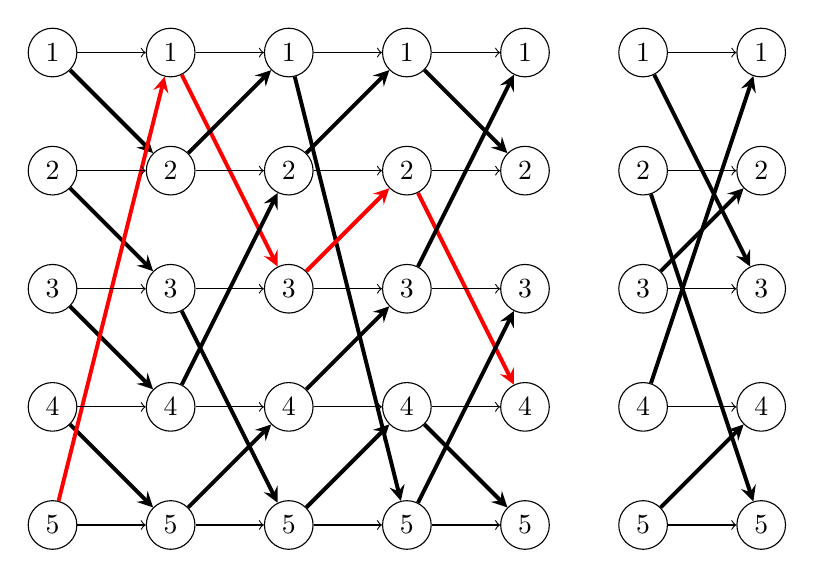
\begin{tikzpicture}[node distance=1.5cm, auto]
\node  (1)[draw, circle, minimum size=0.5cm]  {1};
\node  (2)[draw, circle, minimum size=0.5cm] [  below   of = 1] {2};
\node  (3)[draw, circle, minimum size=0.5cm] [  below  of = 2] {3};
\node  (4)[draw, circle, minimum size=0.5cm] [  below  of = 3] {4};
\node  (5)[draw, circle, minimum size=0.5cm] [  below  of = 4] {5};
\node  (6)[draw, circle, minimum size=0.5cm] [  right   of = 1] {1};
\node  (7)[draw, circle, minimum size=0.5cm] [  right  of = 2] {2};
\node  (8)[draw, circle, minimum size=0.5cm] [  right  of = 3] {3};
\node  (9)[draw, circle, minimum size=0.5cm] [  right  of = 4] {4};
\node  (10)[draw, circle, minimum size=0.5cm] [  right  of = 5] {5};
\node  (11)[draw, circle, minimum size=0.5cm] [  right   of = 6] {1};
\node  (12)[draw, circle, minimum size=0.5cm] [  right  of = 7] {2};
\node  (13)[draw, circle, minimum size=0.5cm] [  right  of = 8] {3};
\node  (14)[draw, circle, minimum size=0.5cm] [  right  of = 9] {4};
\node  (15)[draw, circle, minimum size=0.5cm] [  right  of = 10] {5};
\node  (16)[draw, circle, minimum size=0.5cm] [  right   of = 11] {1};
\node  (17)[draw, circle, minimum size=0.5cm] [  right  of = 12] {2};
\node  (18)[draw, circle, minimum size=0.5cm] [  right  of = 13] {3};
\node  (19)[draw, circle, minimum size=0.5cm] [  right  of = 14] {4};
\node  (20)[draw, circle, minimum size=0.5cm] [  right  of = 15] {5};
\node  (21)[draw, circle, minimum size=0.5cm] [  right   of = 16] {1};
\node  (22)[draw, circle, minimum size=0.5cm] [  right  of = 17] {2};
\node  (23)[draw, circle, minimum size=0.5cm] [  right  of = 18] {3};
\node  (24)[draw, circle, minimum size=0.5cm] [  right  of = 19] {4};
\node  (25)[draw, circle, minimum size=0.5cm] [  right  of = 20] {5};
\node  (26)[draw, circle, minimum size=0.5cm] [  right   of = 21] {1};
\node  (27)[draw, circle, minimum size=0.5cm] [  right  of = 22] {2};
\node  (28)[draw, circle, minimum size=0.5cm] [  right  of = 23] {3};
\node  (29)[draw, circle, minimum size=0.5cm] [  right  of = 24] {4};
\node  (30)[draw, circle, minimum size=0.5cm] [  right  of = 25] {5};
\node  (31)[draw, circle, minimum size=0.5cm] [  right   of = 26] {1};
\node  (32)[draw, circle, minimum size=0.5cm] [  right  of = 27] {2};
\node  (33)[draw, circle, minimum size=0.5cm] [  right  of = 28] {3};
\node  (34)[draw, circle, minimum size=0.5cm] [  right  of = 29] {4};
\node  (35)[draw, circle, minimum size=0.5cm] [  right  of = 30] {5};
\draw[arrows=-stealth, line width=0.5mm] (1) -- (7);
\draw[arrows=-stealth, line width=0.5mm] (2) -- (8);
\draw[arrows=-stealth, line width=0.5mm] (3) -- (9);
\draw[arrows=-stealth, line width=0.5mm] (4) -- (10);
\draw[arrows=-stealth, line width=0.5mm, color=red] (5) -- (6);
\draw[arrows=-stealth, line width=0.5mm, color=red] (6) -- (13);
\draw[arrows=-stealth, line width=0.5mm] (7) -- (11);
\draw[arrows=-stealth, line width=0.5mm] (8) -- (15);
\draw[arrows=-stealth, line width=0.5mm] (9) -- (12);
\draw[arrows=-stealth, line width=0.5mm] (10) -- (14);
\draw[arrows=-stealth, line width=0.5mm] (11) -- (20);
\draw[arrows=-stealth, line width=0.5mm] (12) -- (16);
\draw[arrows=-stealth, line width=0.5mm, color=red] (13) -- (17);
\draw[arrows=-stealth, line width=0.5mm] (14) -- (18);
\draw[arrows=-stealth, line width=0.5mm] (15) -- (19);
\draw[arrows=-stealth, line width=0.5mm] (16) -- (22);
\draw[arrows=-stealth, line width=0.5mm, color=red] (17) -- (24);
\draw[arrows=-stealth, line width=0.5mm] (18) -- (21);
\draw[arrows=-stealth, line width=0.5mm] (19) -- (25);
\draw[arrows=-stealth, line width=0.5mm] (20) -- (23);
\draw[arrows=-stealth, line width=0.5mm] (26) -- (33);
\draw[arrows=-stealth, line width=0.5mm] (27) -- (35);
\draw[arrows=-stealth, line width=0.5mm] (28) -- (32);
\draw[arrows=-stealth, line width=0.5mm] (29) -- (31);
\draw[arrows=-stealth, line width=0.5mm] (30) -- (34);
\draw[->] (1) -- (6);
\draw[->] (2) -- (7);
\draw[->] (3) -- (8);
\draw[->] (4) -- (9);
\draw[->] (5) -- (10);
\draw[->] (6) -- (11);
\draw[->] (7) -- (12);
\draw[->] (8) -- (13);
\draw[->] (9) -- (14);
\draw[->] (10) -- (15);
\draw[->] (11) -- (16);
\draw[->] (12) -- (17);
\draw[->] (13) -- (18);
\draw[->] (14) -- (19);
\draw[->] (15) -- (20);
\draw[->] (16) -- (21);
\draw[->] (17) -- (22);
\draw[->] (18) -- (23);
\draw[->] (19) -- (24);
\draw[->] (20) -- (25);
\draw[->] (26) -- (31);
\draw[->] (27) -- (32);
\draw[->] (28) -- (33);
\draw[->] (29) -- (34);
\draw[->] (30) -- (35);
\end{tikzpicture}
}
\end{frame}



\begin{frame}{Barrington Theorem}
\begin{block}{Theorem 1}
Für jede zyklische Permutation auf [5] $\sigma$ und für jedes DeMorgan Schaltkreis der Tiefe d, die entsprechende Boolesche Funktion kann dank einem 5-PBP der Tiefe höchstens $4^d$ $\sigma$-berechnet werden.
\end{block}
$Beweis$: Durch Induktion über $d$.\\
IA: Für d = 0 $\Rightarrow$ der Schaltkreis ist entweder die Variable $x$ oder ihre Negation $\lnot x$. Für $f(x)$ = $x$ wurde ein Beispiel gegeben und nach dem Satz 2 können wir ein 5-PBP konstruieren, welches $f(x)$ = $\lnot x$ berechnet.\\


\end{frame}
\begin{frame}{Barrington Theorem}
IS: Für d $\ge$ 1. Nach dem Satz 3 können wir annehmen, dass $f$ = $g\wedge h$, wobei $g$ und $h$ Formeln deren Tiefe $d$ - 1 und deren 5-PBP (nach der Induktion Hypothese) $G$ und $H$ haben höchsten die Tiefe $4^{d-1}$. \\
Nach dem Satz 1 können wir annehmen, dass $G$ $\sigma$-$berechnet$ $g$ und $H$ $\tau$-$berechnet$ $h$. Nach dem Satz 3 existiert ein 5-PBP mit der Tiefe 2($size(G)$ + $size(H)$) $\le$ $4^{d}$, welches 
$\sigma\tau\sigma^{-1}\tau^{-1}$-$berechnet$ $f$. Nach dem Satz 4 ist dies eine zyklische Permutation $\Box$. 
\end{frame}

\begin{frame}{Barrington Theorem}
w-Permutation Branching-Programm zu BP umwandeln:\\[4pt]

\only<1>{
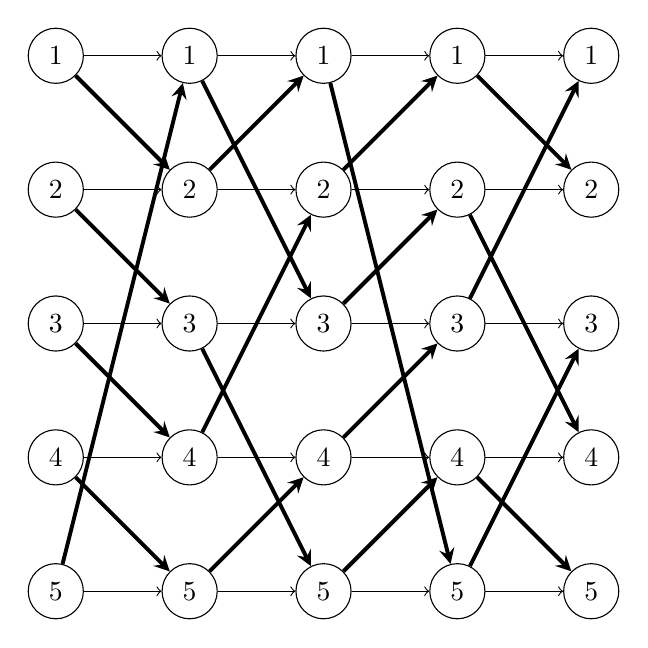
\begin{tikzpicture}[node distance=1.7cm, auto]
\node  (1)[draw, circle, minimum size=0.7cm]  {1};
\node  (2)[draw, circle, minimum size=0.7cm] [  below   of = 1] {2};
\node  (3)[draw, circle, minimum size=0.7cm] [  below  of = 2] {3};
\node  (4)[draw, circle, minimum size=0.7cm] [  below  of = 3] {4};
\node  (5)[draw, circle, minimum size=0.7cm] [  below  of = 4] {5};
\node  (6)[draw, circle, minimum size=0.7cm] [  right   of = 1] {1};
\node  (7)[draw, circle, minimum size=0.7cm] [  right  of = 2] {2};
\node  (8)[draw, circle, minimum size=0.7cm] [  right  of = 3] {3};
\node  (9)[draw, circle, minimum size=0.7cm] [  right  of = 4] {4};
\node  (10)[draw, circle, minimum size=0.7cm] [  right  of = 5] {5};
\node  (11)[draw, circle, minimum size=0.7cm] [  right   of = 6] {1};
\node  (12)[draw, circle, minimum size=0.7cm] [  right  of = 7] {2};
\node  (13)[draw, circle, minimum size=0.7cm] [  right  of = 8] {3};
\node  (14)[draw, circle, minimum size=0.7cm] [  right  of = 9] {4};
\node  (15)[draw, circle, minimum size=0.7cm] [  right  of = 10] {5};
\node  (16)[draw, circle, minimum size=0.7cm] [  right   of = 11] {1};
\node  (17)[draw, circle, minimum size=0.7cm] [  right  of = 12] {2};
\node  (18)[draw, circle, minimum size=0.7cm] [  right  of = 13] {3};
\node  (19)[draw, circle, minimum size=0.7cm] [  right  of = 14] {4};
\node  (20)[draw, circle, minimum size=0.7cm] [  right  of = 15] {5};
\node  (21)[draw, circle, minimum size=0.7cm] [  right   of = 16] {1};
\node  (22)[draw, circle, minimum size=0.7cm] [  right  of = 17] {2};
\node  (23)[draw, circle, minimum size=0.7cm] [  right  of = 18] {3};
\node  (24)[draw, circle, minimum size=0.7cm] [  right  of = 19] {4};
\node  (25)[draw, circle, minimum size=0.7cm] [  right  of = 20] {5};

\draw[arrows=-stealth, line width=0.5mm] (1) -- (7);
\draw[arrows=-stealth, line width=0.5mm] (2) -- (8);
\draw[arrows=-stealth, line width=0.5mm] (3) -- (9);
\draw[arrows=-stealth, line width=0.5mm] (4) -- (10);
\draw[arrows=-stealth, line width=0.5mm] (5) -- (6);
\draw[arrows=-stealth, line width=0.5mm] (6) -- (13);
\draw[arrows=-stealth, line width=0.5mm] (7) -- (11);
\draw[arrows=-stealth, line width=0.5mm] (8) -- (15);
\draw[arrows=-stealth, line width=0.5mm] (9) -- (12);
\draw[arrows=-stealth, line width=0.5mm] (10) -- (14);
\draw[arrows=-stealth, line width=0.5mm] (11) -- (20);
\draw[arrows=-stealth, line width=0.5mm] (12) -- (16);
\draw[arrows=-stealth, line width=0.5mm] (13) -- (17);
\draw[arrows=-stealth, line width=0.5mm] (14) -- (18);
\draw[arrows=-stealth, line width=0.5mm] (15) -- (19);
\draw[arrows=-stealth, line width=0.5mm] (16) -- (22);
\draw[arrows=-stealth, line width=0.5mm] (17) -- (24);
\draw[arrows=-stealth, line width=0.5mm] (18) -- (21);
\draw[arrows=-stealth, line width=0.5mm] (19) -- (25);
\draw[arrows=-stealth, line width=0.5mm] (20) -- (23);
\draw[->] (1) -- (6);
\draw[->] (2) -- (7);
\draw[->] (3) -- (8);
\draw[->] (4) -- (9);
\draw[->] (5) -- (10);
\draw[->] (6) -- (11);
\draw[->] (7) -- (12);
\draw[->] (8) -- (13);
\draw[->] (9) -- (14);
\draw[->] (10) -- (15);
\draw[->] (11) -- (16);
\draw[->] (12) -- (17);
\draw[->] (13) -- (18);
\draw[->] (14) -- (19);
\draw[->] (15) -- (20);
\draw[->] (16) -- (21);
\draw[->] (17) -- (22);
\draw[->] (18) -- (23);
\draw[->] (19) -- (24);
\draw[->] (20) -- (25);

\end{tikzpicture}
}

\only<2>{
\begin{tikzpicture}[node distance=1.5cm, auto]
\node  (1)[draw, circle, minimum size=0.5cm, color=green]  {S};

\node  (6)[draw, circle, minimum size=0.5cm] [  right   of = 1] {1};
\node  (7)[draw, circle, minimum size=0.5cm] [  right  of = 2] {2};

\node  (11)[draw, circle, minimum size=0.5cm] [  right   of = 6] {1};
\node  (12)[draw, circle, minimum size=0.5cm] [  right  of = 7] {2};
\node  (13)[draw, circle, minimum size=0.5cm] [  right  of = 8] {3};

\node  (16)[draw, circle, minimum size=0.5cm] [  right   of = 11] {1};
\node  (17)[draw, circle, minimum size=0.5cm] [  right  of = 12] {2};
\node  (18)[draw, circle, minimum size=0.5cm] [  right  of = 13] {3};

\node  (20)[draw, circle, minimum size=0.5cm] [  right  of = 15] {5};
\node  (21)[draw, circle, minimum size=0.5cm] [  right   of = 16] {1};
\node  (22)[draw, circle, minimum size=0.5cm] [  right  of = 17] {2};
\node  (23)[draw, circle, minimum size=0.5cm] [  right  of = 18] {3};
\node  (24)[draw, circle, minimum size=0.5cm] [  right  of = 19] {4};
\node  (25)[draw, circle, minimum size=0.5cm] [  right  of = 20] {5};

\draw[arrows=-stealth, line width=0.5mm] (1) -- (7);

\draw[arrows=-stealth, line width=0.5mm] (6) -- (13);
\draw[arrows=-stealth, line width=0.5mm] (7) -- (11);

\draw[arrows=-stealth, line width=0.5mm] (11) -- (20);
\draw[arrows=-stealth, line width=0.5mm] (12) -- (16);
\draw[arrows=-stealth, line width=0.5mm] (13) -- (17);

\draw[arrows=-stealth, line width=0.5mm] (16) -- (22);
\draw[arrows=-stealth, line width=0.5mm] (17) -- (24);
\draw[arrows=-stealth, line width=0.5mm] (18) -- (21);

\draw[arrows=-stealth, line width=0.5mm] (20) -- (23);
\draw[->] (1) -- (6);

\draw[->] (6) -- (11);
\draw[->] (7) -- (12);

\draw[->] (11) -- (16);
\draw[->] (12) -- (17);
\draw[->] (13) -- (18);

\draw[->] (16) -- (21);
\draw[->] (17) -- (22);
\draw[->] (18) -- (23);

\draw[->] (20) -- (25);

\end{tikzpicture}
}


\only<3>{
\begin{tikzpicture}[node distance=1.5cm, auto]
\node  (1)[draw, circle, minimum size=0.5cm, color=green]  {S};

\node  (6)[draw, circle, minimum size=0.5cm] [  right   of = 1] {};
\node  (7)[draw, circle, minimum size=0.5cm] [  right  of = 2] {};

\node  (11)[draw, circle, minimum size=0.5cm] [  right   of = 6] {};
\node  (12)[draw, circle, minimum size=0.5cm] [  right  of = 7] {};
\node  (13)[draw, circle, minimum size=0.5cm] [  right  of = 8] {};

\node  (16)[draw, circle, minimum size=0.5cm] [  right   of = 11] {};
\node  (17)[draw, circle, minimum size=0.5cm] [  right  of = 12] {};
\node  (18)[draw, circle, minimum size=0.5cm] [  right  of = 13] {};

\node  (20)[draw, circle, minimum size=0.5cm] [  right  of = 15] {};
\node  (21)[draw, circle, minimum size=0.5cm] [  right   of = 16] {};
\node  (22)[draw, circle, minimum size=0.5cm] [  right  of = 17] {};
\node  (23)[draw, circle, minimum size=0.5cm, color=green] [  right  of = 18] {t};
\node  (24)[draw, circle, minimum size=0.5cm] [  right  of = 19] {};
\node  (25)[draw, circle, minimum size=0.5cm] [  right  of = 20] {};

\draw[arrows=-stealth, line width=0.5mm] (1) -- (7);

\draw[arrows=-stealth, line width=0.5mm] (6) -- (13);
\draw[arrows=-stealth, line width=0.5mm] (7) -- (11);

\draw[arrows=-stealth, line width=0.5mm] (11) -- (20);
\draw[arrows=-stealth, line width=0.5mm] (12) -- (16);
\draw[arrows=-stealth, line width=0.5mm] (13) -- (17);

\draw[arrows=-stealth, line width=0.5mm] (16) -- (22);
\draw[arrows=-stealth, line width=0.5mm] (17) -- (24);
\draw[arrows=-stealth, line width=0.5mm] (18) -- (21);

\draw[arrows=-stealth, line width=0.5mm] (20) -- (23);
\draw[->] (1) -- (6);

\draw[->] (6) -- (11);
\draw[->] (7) -- (12);

\draw[->] (11) -- (16);
\draw[->] (12) -- (17);
\draw[->] (13) -- (18);

\draw[->] (16) -- (21);
\draw[->] (17) -- (22);
\draw[->] (18) -- (23);

\draw[->] (20) -- (25);

\end{tikzpicture}
}

\end{frame}

\end{document}
